%% For double-blind review submission, w/o CCS and ACM Reference (max 
%%submission space)
\documentclass[sigplan,review,anonymous]{acmart}\settopmatter{printfolios=true,printccs=false,printacmref=false}
%% For double-blind review submission, w/ CCS and ACM Reference
%\documentclass[sigplan,review,anonymous]{acmart}\settopmatter{printfolios=true}
%% For single-blind review submission, w/o CCS and ACM Reference (max 
%%submission space)
%\documentclass[sigplan,review]{acmart}\settopmatter{printfolios=true,printccs=false,printacmref=false}
%% For single-blind review submission, w/ CCS and ACM Reference
%\documentclass[sigplan,review]{acmart}\settopmatter{printfolios=true}
%% For final camera-ready submission, w/ required CCS and ACM Reference
%\documentclass[sigplan]{acmart}\settopmatter{}

\usepackage{soul}

%\usepackage{booktabs} % For formal tables
%\documentclass{article}
%\usepackage{floatrow}
\usepackage{rotating}
\usepackage{graphicx}
\usepackage{multirow}
%\usepackage[dvipsnames]{xcolor}
\usepackage{amsfonts}
\usepackage{amsmath}
\usepackage{amssymb}
\usepackage{mathtools}
\usepackage{wrapfig}
\usepackage{listings}
\usepackage{graphicx}
\usepackage{caption}
\usepackage{tabularx}
%\usepackage{amsthm}
%\usepackage[section]{placeins}
\usepackage{enumitem}
%\usepackage[a4paper, total={7in, 10.5in}]{geometry}
\usepackage[font={small}]{caption}
%\usepackage[font={bf,sf,small}]{caption}
%\usepackage[linesnumbered,ruled]{algorithm2e}
\usepackage{algpseudocode}
\captionsetup{labelfont=bf,textfont=bf}
\usepackage[font={bf,sf,scriptsize}]{subfig} 
\usepackage{amsthm}

%
%\usepackage[utf8]{inputenc}
%\usepackage{url}
%\usepackage{amsmath,amsthm,amssymb,amsfonts}
\usepackage{algorithm}
\usepackage{algpseudocode}
\usepackage{algorithmicx}
%\usepackage{graphicx}
%\usepackage{caption}
%\usepackage[thinlines]{easytable}
%\usepackage{pdfpages}
%\usepackage{fancyhdr}
%\usepackage{booktabs}
%\usepackage{footnote}
%\usepackage{footmisc}
%\usepackage{mathtools}
%\usepackage{multirow}
%%\usepackage{siunitx}
%%\usepackage{booktabs}
%%\usepackage{blindtext}
%%\usepackage[pdfencoding=auto,psdextra]{hyperref}
%
%\fancyhf{}
%\renewcommand{\headrulewidth}{0pt}
%\renewcommand{\footrulewidth}{0pt}
%
%\DeclarePairedDelimiter\abs{\lvert}{\rvert}
%
%\makeatletter
%\let\oldabs\abs
%\def\abs{\@ifstar{\oldabs}{\oldabs*}}
%\makeatother
%\def\E{\mathbb{E}}
%
%\makeatletter
%\g@addto@macro \normalsize {%
%	\setlength\abovedisplayskip{5pt plus 2pt minus 2pt}%
%	\setlength\belowdisplayskip{5pt plus 2pt minus 2pt}%
%}
%\makeatother


\renewcommand{\algorithmicrequire}{\textbf{Input:}}
\renewcommand{\algorithmicensure}{\textbf{Output:}}

\newcommand\numberthis{\addtocounter{equation}{1}\tag{\theequation}}
\def\NoNumber#1{{\def\alglinenumber##1{}\State #1}\addtocounter{ALG@line}{-1}}



%\usepackage[demo]{graphicx}
%\setlength{\footskip}{15pt}
%\usepackage[utf8]{inputenc}
%\usepackage[english]{babel}
\newtheorem{theorem}{Theorem}[section]
\newtheorem*{corollary*}{Corollary}
\newtheorem{corollary}{Corollary}[theorem]
%\newtheorem{lemma}[theorem]{Lemma}
\newcommand\todo[1]{\textcolor{red}{#1}}
\newcommand\greg[1]{\textcolor{blue}{[Greg: #1]}}
\newcommand\toskip[1]{\textcolor{green}{[possibly to skip: #1]}}
\newcommand\mac[1]{\textcolor{red}{[Mac: #1]}}

\newcommand*\diff{\mathop{}\!\mathrm{d}}
\newcommand*\Diff[1]{\mathop{}\!\mathrm{d^#1}}

\DeclareMathOperator*{\argmax}{arg\,max}
\DeclareMathOperator*{\argmin}{arg\,min}

%  \lstset{language=C,
%    keepspaces=true,
%    frame=tb,
%    basicstyle=\ttfamily,
%    columns=fixed,
%    morekeywords={enddo},
%    mathescape}

\lstset{language=C,
        escapechar=|,
        keepspaces=false,
        frame=tb,
        framexleftmargin=1.5em,
        basicstyle=\tt\scriptsize,
        columns=fixed,
        %otherkeywords={enddo,forall,bool,true,false, int64_t, MPI_Op, in, parallel, function},
        otherkeywords={enddo,end,forall,bool,true,false, int64_t, MPI_Op, function},
        tabsize=2,
        breaklines=true,
        captionpos=b,
        %aboveskip=-1.5em,
        %belowskip=-0.5em,
        numbers=left,
        xleftmargin=1.5em,
        keywordstyle=\bfseries\color{black!400!black},
        stringstyle=\color{orange},
        commentstyle=\color{darkgrey},
        numberstyle=\scriptsize,numbersep=3pt,mathescape}

\usepackage{cleveref}
\usepackage[utf8]{inputenc}
\crefname{section}{§}{§§}
\Crefname{section}{§}{§§}

\newtheorem{defn}{Definition}
\newtheorem{thm}{Theorem}
\newtheorem{clm}{Claim}
\newtheorem{crl}{Corollary}
\newtheorem{lma}{Lemma}
%\newtheorem{proof}{Proof}
%\newtheorem*{proof*}{Proof}
\newtheorem{observation}{Observation}

\newcommand{\macb}[1]{\textbf{\textsf{#1}}}

\DeclareSymbolFont{matha}{OML}{txmi}{m}{it}% txfonts
\DeclareMathSymbol{\varS}{\mathord}{matha}{83}

\acmConference[PPoPP'19]{ACM SIGPLAN Annual Symposium on Principles and 
Practice of Parallel Programming}{February 16--20, 2019}{Washington DC, USA}
% \acmYear{}
% \acmISBN{} 
% \acmDOI{}
\startPage{1}

%% Copyright information
%% Supplied to authors (based on authors' rights management selection;
%% see authors.acm.org) by publisher for camera-ready submission;
%% use 'none' for review submission.
\setcopyright{none}
%\setcopyright{acmcopyright}
%\setcopyright{acmlicensed}
%\setcopyright{rightsretained}
%\copyrightyear{2018}           %% If different from \acmYear

%% Some recommended packages.
\usepackage{booktabs} 
\usepackage{makecell}
\hypersetup{draft}

\usepackage{pifont}

\begin{document}

%% Title information

\title[I/O-Optimal Dimensionless Matrix Multiplication]{Breaking The 
Monopoly of Dimensions: Towards I/O-Optimal Matrix Multiplication}


\author{First1 Last1}
\authornote{with author1 note}          %% \authornote is optional;
                                        %% can be repeated if necessary
\orcid{nnnn-nnnn-nnnn-nnnn}             %% \orcid is optional
\affiliation{
  \position{Position1}
  \department{Department1}              %% \department is recommended
  \institution{Institution1}            %% \institution is required
  \streetaddress{Street1 Address1}
  \city{City1}
  \state{State1}
  \postcode{Post-Code1}
  \country{Country1}                    %% \country is recommended
}
\email{first1.last1@inst1.edu}          %% \email is recommended

%% Author with two affiliations and emails.
\author{First2 Last2}
\authornote{with author2 note}          %% \authornote is optional;
                                        %% can be repeated if necessary
\orcid{nnnn-nnnn-nnnn-nnnn}             %% \orcid is optional
\affiliation{
  \position{Position2a}
  \department{Department2a}             %% \department is recommended
  \institution{Institution2a}           %% \institution is required
  \streetaddress{Street2a Address2a}
  \city{City2a}
  \state{State2a}
  \postcode{Post-Code2a}
  \country{Country2a}                   %% \country is recommended
}
\email{first2.last2@inst2a.com}         %% \email is recommended
\affiliation{
  \position{Position2b}
  \department{Department2b}             %% \department is recommended
  \institution{Institution2b}           %% \institution is required
  \streetaddress{Street3b Address2b}
  \city{City2b}
  \state{State2b}
  \postcode{Post-Code2b}
  \country{Country2b}                   %% \country is recommended
}
\email{first2.last2@inst2b.org}         %% \email is recommended



\begin{abstract}
%
\greg{Old sketch of the abstract. To be done at the end}
%
In this paper we address an allegedly well-known problem of distributed Matrix
Matrix Multiplication and show new optimizations both from theoretical and
implementation sides. We establish a new framework for assessing analytical
data movement lower bounds, together with deriving optimal sequential and
parallel scheduling. Our "bottom-up" parallelization technique, opposed to
state of the art "top-down" approaches is naturally agnostic to problem
dimensions and is provably optimal in all scenarios, resulting in up to
$\sqrt{3}$ times reduction in communication volume. With our fine-tuned data
layout transformations, we are able to achieve X \% peak FLOP/s running on up
to Y nodes on the Piz Daint supercomputer, beating currently fastest-known
algorithms by a factor of Z, using provably I/O optimal, robust schedule and
employing RDMA mechanisms for communication-computation overlap.
%
%Based on an existing pebble game abstraction, we come to fundamental
%observations about parallel scheduling and data reuse, deriving new tiling
%scheme for Matrix-Matrix Multiplication, achieving a tight bound of
%$\frac{2mnk}{\sqrt{S}}$ I/O operations. We show the new NP-hardness proof for
%I/O optimal scheduling.
%
\end{abstract}


\keywords{I/O complexity, scheduling, pebble games}

%% \maketitle
%% Note: \maketitle command must come after title commands, author
%% commands, abstract environment, Computing Classification System
%% environment and commands, and keywords command.
\maketitle

\section{Introduction}
\label{sec:intro}

%To-G: One paragraph must serve *one* specific goal that one must be able to
%state in one short (~10 words at most) sentence. The previous intro was one
%large bulk of text - not good. I split into paragraphs below. Double check if
%you understand *exactly* why the division into paragraphs is like 
%this.
%\begin{figure*}[!tbp]
%  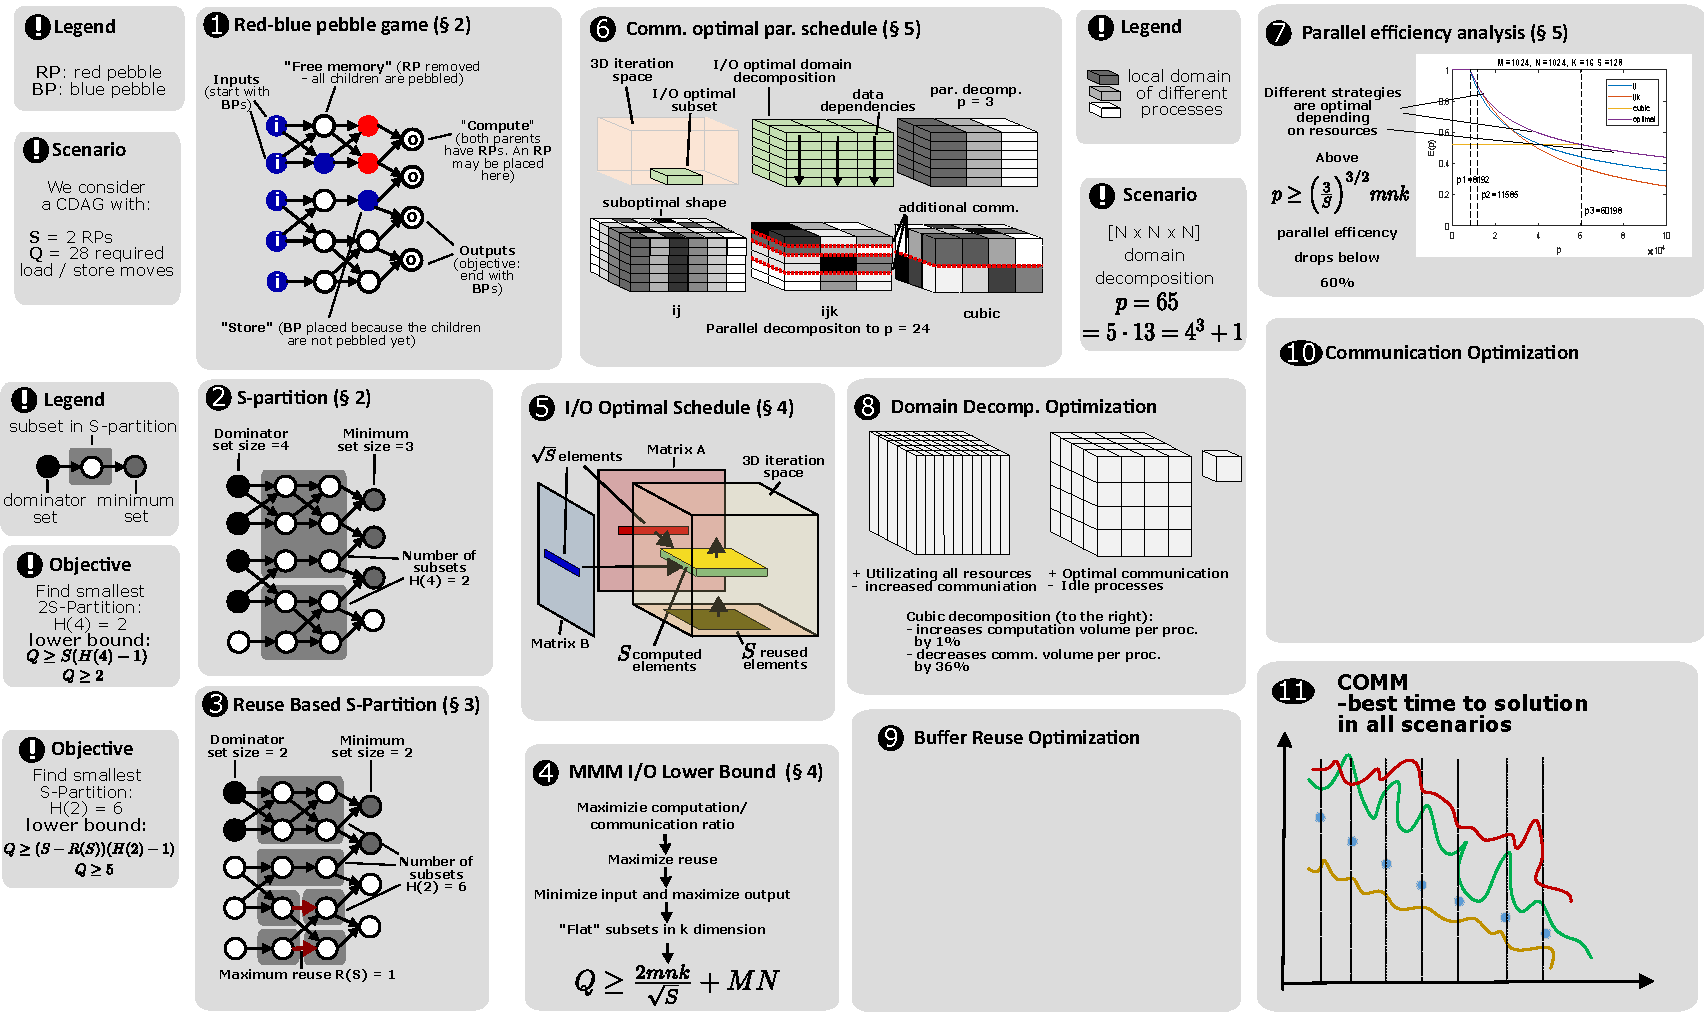
\includegraphics[width=\textwidth]{figures/paperOrganization}
%  \caption{Achieving data movement optimal MMM in eleven simple 
%    steps: (I) I/O lower bounds and red-blue pebble game, (II) 
%    $2S$-partition lemma, (III) reuse-based lemma, (IV) MMM I/O 
%    lower 
%    bound, (V) I/O optimal schedule, (VI) communication optimal 
%    parallel schedule, (VII) parallel efficiency analysis, (VIII) 
%    buffer optimization, (IX) communication optimization, (X) 
%    process 
%    decomposition optimization, (XI) best time-to-solution 
%    result. }
%  %
%  \label{fig:paperOrganization}
%\end{figure*}

Matrix-matrix multiplication (MMM) is one of the most fundamental building
blocks in scientific computing. It is widely used not only in virtually all
linear algebra algorithms (Cholesky and LU
decomposition~\cite{meyer2000matrix}, eigenvalue
factorization~\cite{chatelin2012eigenvalues}, triangular
solvers~\cite{linearAlgebraLAPACK}), but also in numerous graph algorithms such
as Breadth-First Search (BFS)~\cite{cormen2009introduction} or Triangle
Counting~\cite{azad2015parallel} through efforts such as
GraphBLAS~\cite{kepner2016mathematical}. Other use cases include spectral
clustering~\cite{ng2002spectral} or machine
learning~\cite{abadi2016tensorflow}.  Thus, accelerating MMM routines is of
great significance for many domains.

Hong and Kung~\cite{redblue} proved nearly 30 years ago a sequential I/O lower
bound for matrix multiplication to be $\Omega\left(\frac{n^3}{\sqrt{S}}\right)$
in their two-level memory model, where $S$
is the size of the fast memory
%
\footnote{Throughout this paper we use the original notation from Hong and Kung 
to denote the memory size $S$. In literature, it is also common to use the 
symbol $M$~\cite{externalMem,IronyMMM, parallelExMem}.} 
%	and denote the memory size $M$. Hong and Kung used the symbol $S$.}. 
	Irony et al.~\cite{IronyMMM} extended those
results to the parallel machine with $p$ processes,
each of which has a fast private memory of size~$S$, proving the
$\Omega\left(\frac{n^3}{p\sqrt{S}}\right)$ bound on communication per process.
%
%Various optimizations 
%Ever since then, those bounds serve as a
%driving force in developing better algorithms. \mac{This sounds a bit weird -
%why are the bounds a driving force? You can also see them as, well, bounds? I
%would probably remove it} This evolution includes optimizations like
%parallelization~\cite{parallelMMM}, tiling~\cite{tiling}, 2D~\cite{summa} and
%3D~\cite{summa3d} domain decomposition or data layout
%optimization~\cite{scalapackLayout}.
%
If the memory size~$S$ is bounded by the size the
input data ($pS = \mathcal{O}(n^2)$), the bound
$\mathcal{O}\left(\frac{n^2}{\sqrt{p}}\right)$  is asymptotically attainable by
algorithms such as Cannon's~\cite{Cannon} or SUMMA~\cite{summa}. In the
presence of extra memory ($pS = \mathcal{O}(p^{1/3} n^2)$), the 3D
decomposition~\cite{summa3d} yields a better asymptotic bound
$\mathcal{O}\left(\frac{n^2}{P^{2/3}}\right)$. The 2.5D algorithm by Solomonik
and Demmel~\cite{25d} effectively interpolates
between those two results, depending on the available
memory.

Another class of optimizations, based on group theory,
are Strassen-like routines~\cite{Strassen}, which asymptotically reduce the
number of arithmetic operations. Currently, the algorithm with the lowest
asymptotic complexity $O(n^{2.3729}$) is by Le~Gall~\cite{LeGall}. In our work,
however, we focus only on the ``classical'' MMM algorithms which perform $n^3$
additions and multiplications, as they are often faster in practice on modern 
parallel architectures with deep memory hierarchies~\cite{strassenVsClassic}.  

While the largest focus has traditionally been
placed on accelerating the multiplication of square matrices, more focus has
recently been put on
non-square matrices as well. Such scenarios are common in a number of
relevant areas and problems, for example in machine learning
\cite{rectangularML} or computational chemistry~\cite{rectangularChemistry}.
%
Unfortunately, it has been shown
that algorithms optimized for squared matrices often perform poorly in cases
when matrix sizes vary significantly~\cite{CARMA}. 
%
This issue is tackled in the work by Demmel et al.~\cite{CARMA}, who introduced
CARMA, an algorithm that achieves asymptotic lower bounds for all
configurations of dimensions and memory size.  

%\mac{You must mention CTF after
%this e-mail exchange with Edgar} \greg{I need results from Marko}

%
%\mac{This ``intra-node memory sizes'' comes out of the blue - why do we care?
%So far, you only motivated shapes. If this memory size parameter is crucial
%for later sections, I would also suggest a small paragraph for this, with
%concrete examples on why it matters}\greg{changed to just "memory" and there
%are referenced to this}

However, we observe several problems of the current state-of-the art
algorithms, such as ScaLAPACK~\cite{scalapack} (an implementation of
SUMMA), Cyclops Tensor Framework (CTF)~\cite{cyclops} (an implementation of the 
2.5D MMM algorithm), or CARMA~\cite{CARMA}. ScaLAPACK supports
only the 2D~decomposition  and requires a user to
fine-tune parameters such as block sizes or process
decomposition. CTF yields poor performance on matrices with 
dimensions which are multiples of large primes
\greg{this is what preliminary results show. Waiting for full results}, a 
common case in, e.g,
computational chemistry~\cite{joost}. Moreover, the recursive
implementation of CARMA cannot directly handle scenarios when the number of
processes is not the power of two, a common
case, as the number of processes is usually determined by the available
hardware resources, rarely a power of two.  For example Piz Daint, the
third fastest supercomputer in 2017, has 1,813 CPU nodes, which are
impossible to arrange in a cubic grid. Furthermore,we emphasize that asymptotic 
complexity is an insufficient measure of speedup. For example, the
Coppersmith--Winograd algorithm~\cite{coppersmith} achieves computational
complexity of $\mathcal{O}(n^{2.376})$, but its constant terms are 
prohibitively big and
make it slower in practice than the classical $\mathcal{O}(n^{3})$ algorithms. 
We later (\cref{sec:evaluation}) show that CARMA suffers from similar
overheads.




%%
%, a common case in practice
%\mac{Again, at least one sentence to this. Why not suitable? What happens?
%'Unsuitable - extremely confusing word...}. For example, Del Ben et
%al.~\cite{joost} used the "tall and skinny" matrices to simulate water
%molecules' interaction \mac{This sentence is completely out of the place. You
%just finished writing about why CARMA and others are bad. And suddenly an
%example of using tall and skinny matrices. Must go elsewhere}. Matrix dimension
%sizes are determined by their number - e.g., for 64 molecules, M=n=8704 and
%k=933888 \mac{Some comment as above - this must go elsewhere}. The number of
%processes, on the other hand, is often determined by available resources and is
%rarely a divisor of the problem size. 

In this work, we present COMM (Communication Optimal Matrix Multiplication): 
an algorithm that takes a new approach to multiplying
matrices and alleviates the above issues. COMM is I/O optimal \emph{with regard 
to all constant factors}
for all combinations of parameters.
%
To prove the optimality of our algorithm,  we (1) first provide a new 
constructive proof of sequential I/O lower bound, improving the constant 
factors of an existing bound 
by Smith and van de Gein~\cite{tightMMM}, (2) derive the communication cost of  
parallelizing the sequential
schedule, (3) construct a
communication optimal parallel schedule. 
or SUMMA~\cite{summa}. The detailed communication analysis of COMM, 2D, 3D and 
recursive decompositions is
presented in Table~\ref{tab:summary}. Our algorithm reduces the data 
movement volume up to $\sqrt{3} \approx 1.73$ times compared to the 
asymptotically optimal recursive decomposition and up to 
$\max\{n,m,k\}$ times compared to the 2D
algorithms, like Cannon's~\cite{generalCannon} or SUMMA~\cite{summa}.


Unlike CARMA that is based on the recursive data layout, our implementation
enables transparent integration with the ScaLAPACK
format~\cite{scalapackLayout} and delivers near-optimal computation throughput.
%
We later (\cref{sec:implementation}) illustrate that the obtained schedule 
naturally expresses
computation-communication overlap, 
%
%\mac{if it's true, I would also add here
%``unlike the existing approaches''}\greg{not sure about this part}
%
 which can 
be used for even higher speedups
using Remote Direct Memory Access (RDMA) mechanisms.
%
%We further motivate our work in Figure~\ref{fig:motivation-page-1} that shows
%the advantages of our algorithm over the state of the art \greg{what do you 
%want to put here?}.
%%
Our implementation
also uses various techniques, like buffer and layout optimization to further
accelerate the execution time. Finally, our I/O optimal approach is
easily generalizable to other linear algebra kernels. 

We provide the following contributions:

\begin{itemize}[leftmargin=1em]
%
\item We present COMM : the distributed MMM algorithm that is I/O optimal for 
any combination of parameters.
%
%the algorithm achieving up to ?? speedup (?? on average) in
%the total runtime of the MMM scheme over the existing state-of-the-art 
%implementations,
%
\item Extending the general analysis of I/O complexity, we
show a new proof constructive of the sequential MMM I/O lower bound,
delivering tight constant factors (~\cref{sec:seqOptimality}. We extend this 
proof to both distributed and shared memory machines (\cref{sec:parOptimality}),
%
%\item we \mac{We} confront the parallel efficiency of our schedule with 
%existing state-of-the art 2D and 3D matrix
%multiplication variants \mac{state what is the outcome of this confrontation,
%we must contribute sth!} (~\cref{sec:parOptimality} \mac{use cref}),
%
\item We use block-cyclic data layout(~\cref{sec:datalayout}) and a static 
buffer pre-allocation(~\cref{sec:bufferReuse}), which reduce
memory footprint for communication buffers and guarantees minimal reshuffling
of input data, providing better compatibility with ScaLAPACK format than CARMA
(~\cref{sec:implementation}),
%
\item We naturally express the computation-communication overlap, which enables 
even higher speedups by
leveraging the advantages of the RDMA mechanism~(\cref{sec:implementation}),
%
\item We perform extensive evaluation on the Piz Daint supercomputer for an 
extensive selection of problem
dimensions, memory sizes, and numbers of
processes, showing the speedup of up to ?? (?? on average), compared to 
ScaLAPACK, CTF and CARMA (~\cref{sec:evaluation}).
%
\end{itemize}

%
%%
%\mac{Also, see the long comment on top-down above. These 3 reasons here are not
%enough to understand why this thing is called bottom-up.}.
%%
%Our schedule is based on the ``S--partitioning'' concept from the Hong and 
%Kung's 
%red--blue
%pebble game~\cite{redblue} to derive the best (i.e., optimal) partitioning
%routine that minimizes data movement for a given MM product in a parallel
%setting. The model is simplistic and it transparently applies both to 
%distributed and shared memory machines for all possible combinations of 
%parameters.
%%
%We illustrate an intuitive comparison of our bottom-up approach versus the
%classic top-down schemes in Figure~\ref{fig:topdown-vs-bottomup}.

%
%  - \mac{Using such dashes
%is a bad idea in papers, reads bad and informal. Colons are better} it 
%minimizes both the number of I/O 
%operations (vertical data movement across the memory hierarchy) and 
%communication between processes in distributed setting (horizontal data 
%movement) \mac{I thought at this point it's somewhat weird that you combine 
%these two
%and name them in this way. I
%mean, distributed *IS* actually I/O, right? Not disk I/O, but still I/O (NIC, 
%network).
%I would (1) think how to maybe name it a bit better, and (2) investigate
%thoroughly the connection and the overlapping papers}. Our key idea is to 
%``invert'' the traditional ``top-down''
%approach for multiplying matrices, shared by all the mentioned state-of-the-art
%algorithms, that fix the domain partitioning in some predefined fashion
%(2D~\cite{Cannon}, 2.5D~\cite{25d}, or
%recursive~\cite{CARMA}) \mac{The word ``invert'' and ``top-down'' is confusing.
%You just write it down like sth obvious, but it's not obvious (calling all 
%these
%schemes top-down is not obvious). I would suggest to maybe first provide 1-3 
%sentences
%that will straightforwardly explain on why all these schemes are called 
%``top-down'',
%focusing (in this explanation) ALSO on the downsides of this approach. Only 
%after, 
%I would state that we do bottom-up, and invert the top-down, but write it in 
%such
%a way that it is clear WHAT EXACTLY is inverted in the top-down approach}.
%

%
% \mac{Do *not* refer to this figure here. This figure is very very complex and
% long. If you want a simple top-down VS bottom-up figure, it MUST focus ONLY
% on top-down vs bottom-up. Not on everything in the paper...}

\begin{figure}[!tbp]
\centering
%
\subfloat[3D domain
decomposition]{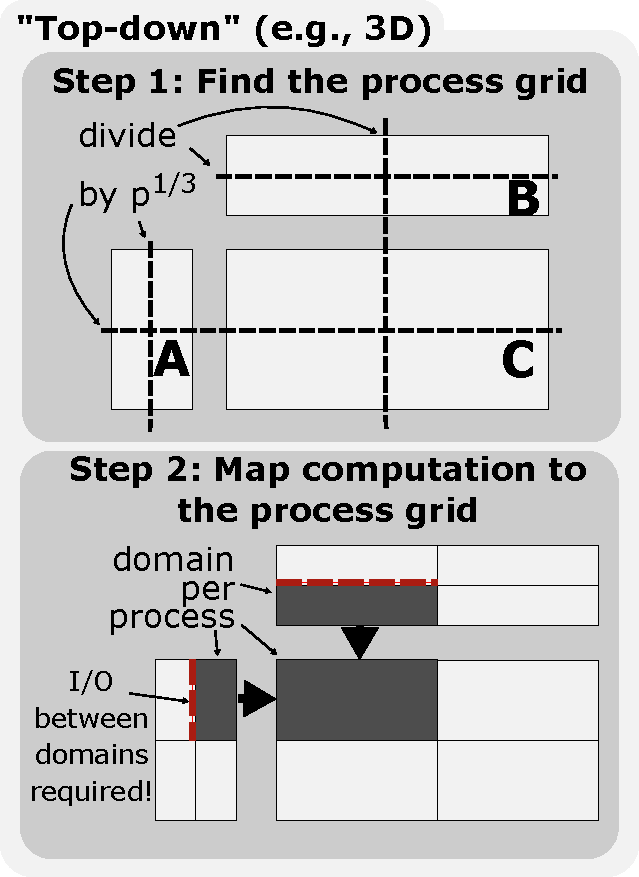
\includegraphics[width=0.22\textwidth]
	{figures/top-down-bottom-up-1}\label{fig:f1}}
%
\hfill
%
\subfloat[COMM decomposition]{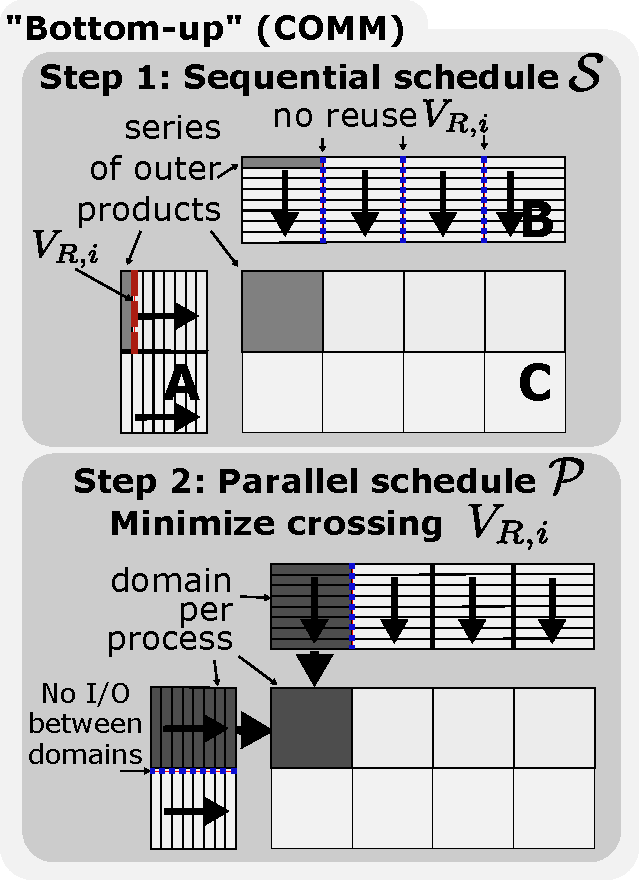
\includegraphics[width=0.22\textwidth]
	{figures/top-down-bottom-up-2}\label{fig:f2}}
%
\caption{Domain decomposition using $p=8$  processes. In 
the scenario (a), a straightforward 3D decomposition divides every dimension in 
$p^{1/3}=2$. In the scenario (b), COMM starts by finding an optimal sequential 
schedule and then parallelizes it minimizing crossing dependencies. The total 
communication volume is reduced by 17\% compared to the former strategy.}
%
\label{fig:topdown-vs-bottomup}
\end{figure}


\begin{table*}
%
\setlength{\tabcolsep}{4pt}
\renewcommand{\arraystretch}{2}
\centering
%\footnotesize
\scriptsize
\sf
%
\begin{tabular}{lllll}
%
\toprule
%
 & \textbf{2D~\cite{summa}} & \textbf{2.5D~\cite{25d}} & 
 \textbf{CARMA~\cite{CARMA}} & \textbf{Our work~(\cref{sec:seqScheduling} )} \\
%
\midrule
%
\makecell[l]{\textbf{process}\\
\textbf{decomposition} \\
$\left[p_m \times p_n \times p_k\right]$}
&
$\left[\sqrt{p} \times \sqrt{p} \times 1\right]$
&
\makecell[l]{$\left[\sqrt{p/c} \times \sqrt{p/c} \times c\right]$,\\
$c = \frac{pS}{mk + nk}$}
& 
\makecell[l]{$\left[{2^{a_1}} \times {2^{a_2}} \times {2^{a_3}}\right]$,\\
$a_1 + a_2 + a_3 = \log_2(p)$}
& 
\makecell[l]{$\left[\frac{m}{\sqrt{S}} \times \frac{n}{\sqrt{S}} \times 
\frac{k}{d}\right]$,\\
$d = \frac{mnk}{pS}$}
%
\vspace{1.0em}
%
\\
%
%\midrule
%
\textbf{domain size}
&
$\left[\frac{m}{\sqrt{p}} \times \frac{n}{\sqrt{p}} \times k\right]$ 
&
$\left[\frac{m}{\sqrt{p/c}} \times \frac{n}{\sqrt{p/c}} \times 
\frac{k}{c}\right]$
&
$\left[\frac{m}{2^{a_1}} \times \frac{n}{2^{a_1}} \times 
\frac{k}{2^{a_1}}\right]$
& 
$\left[{\sqrt{S}} \times {\sqrt{S}} \times {d}\right]$
%
\vspace{0.5em}
%
\\
%
\midrule
%
\makecell[l]{\textbf{communication}\\
\textbf{volume}}
&
$\frac{1}{\sqrt{p}} \left(mk + nk\right)$
&
\makecell[l]{$(mk + nk)\sqrt{\frac{I}{p^2S}} + \frac{MNS}{I}$, \\
$I = mn + mk + nk$}
&
\makecell[l]{$2\min \Big\{\sqrt{3} \frac{mnk}{p\sqrt{S}},
	\left(\frac{mnk}{P}\right)^{2/3} \Big\} $ \\
	$ + \left(\frac{mnk}{P}\right)^{2/3}$}
& 
$\min \Big\{S + 2 \cdot \frac{mnk}{p\sqrt{S}}, 3 
\left(\frac{mnk}{P}\right)^{2/3} \Big\}$
%
\vspace{0.5em}
%
\\
%
\midrule
%
\makecell[l]{\textbf{``the easiest case'':}\\
$m = n = k$,\\
$S = 2\frac{n^2}{p}, p=2^{3n}$}
&
$\frac{2N^2 }{\sqrt{p}}$
&
$\frac{2N^2 }{\sqrt{p}}$
&
$2N^2 \left(\sqrt{\frac{3}{2p}} + \frac{1}{2p^{2/3}} \right)$
& 
$\frac{2N^2 }{\sqrt{p}}$
%
\vspace{1.0em}
%
\\
%
\midrule
%
\makecell[l]{\textbf{``the hardest case'':}\\
$m = n = \sqrt{p}$,\\
$k = \frac{p^{3/2}}{4}$,\\
$S = 2\frac{nk}{p^{2/3}}, p=2^{3n + 1}$}
&
$\frac{p^{3/2}}{2}$
&
$\frac{p^{4/3}}{2} + p^{1/3}$
&
$\frac{3p}{4}$
& 
$\frac{3-2^{1/3}}{2^{4/3}}p \approx 0.69 p$
%
\\
%
\bottomrule
%
\end{tabular}
%
\caption{The formal summary of 2D,
2.5D, CARMA, and COMM schemes for matrix-matrix multiplication (The 3D 
decomposition is a special case of 2.5D, where $c=p^{1/3}$).
The most important symbols used here are described in Table~\ref{tab:symbols}.
The "easiest case" is when the matrices are square and there is no extra
memory for redundant copies of input data. The "hardest case" is when $k \gg m
= n$ and there is space for extra $p^{1/3}$ copies.
For simplicity, we assume that parameters are chosen such that all divisions
have integer results.}
%
\label{tab:summary}
\end{table*}
%
%The overview of the paper's organization is presented in 
%Figure~\ref{fig:paperOrganization}.
%\mac{I would provide at least 2-3 sentences here (if you want to make it a 
%separate
%paragraph), OR merge this one sentence in some other paragraph.}

\section{Background}

In this section, we discuss necessary concepts and terminology needed for our 
analysis. The most important symbols used in the paper are gathered in 
Table~\ref{tab:symbols}.


\begin{table}[h!]
	%
	\centering
	%\footnotesize
	\scriptsize
	%\ssmall
	\sf
	\begin{tabular}{@{}l|ll@{}}
		\toprule
		\multirow{5}{*}{\begin{turn}{90}\textbf{MMM}\end{turn}}
		& $m, n, k$& Matrix dimensions \\
		& $A, B$& Input matrices, $A \in \mathbb{R}^{m \times k}, B \in 
		\mathbb{R}^{k \times n}$ \\
		& $C = AB$& Output matrix, $C \in \mathbb{R}^{m \times n}$ \\
		& $p$& Number of processes \\
		& $S$& Memory size per process \\
		\midrule
		\multirow{11}{*}{\begin{turn}{90}\textbf{I/O complexity 
		(~\cref{sec:introIO})}\end{turn}}
		& $G$&A directed acyclic graph $G=(V,E)$\\
		%& $n,m$&Numbers of vertices and edges in $G$; $|V| = n, |E| = m$.\\
		& $S$ & Number of red pebbles (size of the fast memory)\\
		& $V_i$ & An $i$-th subcomputation of an $S$-partition \\
		& $Dom(V_i), Min(V_i)$ & Dominator and minimum sets of subcomp. 
		$V_i$\\
		& $V_{R,i}$ & Set of vertices containing red pebbles just\\
		& &  before $V_i$ starts and used by $V_i$ (reuse set) \\
		& $H(S)$ & Cardinality of a smallest S-partition \\
		& $R(S)$ & Maximum reuse volume between subcomputations \\
		& $Q$ & Minimal number of I/O operations of any valid \\ 
		& & execution of $G$ \\
				& $\rho_i$ & Computational 
		intensity of $V_i$\\
		\midrule
		\multirow{8}{*}{\begin{turn}{90}
				%
				%\makecell[l]{\textbf{parallel} 
				%	\\ \textbf{scheduling}}
				%
				\textbf{scheduling (~\cref{sec:seqOptimality}, 
				~\cref{sec:parOptimality})}
			\end{turn}} 
		& $\mathcal{V}$ & 3D iteration space of of MMM~\cite{tiling}\\         
		& \textbf{i},\textbf{j},\textbf{k} & orthonormal vectors spanning 
		$\mathcal{V}$\\
		& \textbf{uv} & plane spanned by vectors \textbf{u} and \textbf{v}\\
		& $\phi_{uv}(V)$ & projection of subspace $V$ onto plane \textbf{uv}\\
		& $\mathcal{I}_i$ & Surface of a subcomputation $V_i$ (size of the 
		input)\\
		& $\mathcal{S} = \{V_i\}$ & Sequential schedule (an ordered set of 
		 $V_i$) \\ 
		& $\mathcal{P} = \{\mathcal{S}_j\}$ & Parallel schedule (a set of 
		sequential schedules $\mathcal{S}_i$) \\
		& $W$ & I/O cost of a schedule \\
		\midrule
		
		%\multirow{1}{*}{\begin{turn}{90}\textbf{.}\end{turn}}
		%                    & $S$ & The number of .\\
		\bottomrule
	\end{tabular}
	%\vspace{-0.5em}
	%
	%\vspace{-0.5em}
	%
	\caption{The most important symbols used in the paper.}
	%
	\label{tab:symbols}
	\vspace{-0.5em}
\end{table}
\subsection{Computation Model}

We now briefly specify a model of a \emph{general} computation; we use this
model in both the sequential and parallel setting.

An algorithm is modeled with a computational directed acyclic graph 
(CDAG) $G=(V,E)$~\cite{completeRegisterProblems,pebblegameregister, 
registerpebblecolor}.
First, $V$ is a set of
vertices; one vertex represents one elementary operation in the given
computation. $E$ is a
set of edges; an edge represents a data dependency between operations in
$V$. We call a set of all immediate predecessors (or successors) of a vertex 
its \emph{parents} (or \emph{children}). 
Two selected subsets $I, O \subset V$ are \emph{inputs} and \emph{outputs}, 
that is, sets of vertices that have no parents (or children, 
respectively).
%
A \emph{schedule} is a dependency-preserving sequence of 
elementary operations (ordering of vertices of the CDAG). One schedule 
therefore 
corresponds to one of topological orders of $G$. For example, it is an 
order 
in which all $n^3$ multiplications in MMM are performed.

\subsection{Machine Model}

We use a well-established model for parallel computations with $p$
processes, each with local memory of size $S$ words~\cite{CARMA,25d}).
A process can hold, send, and receive from any other process up to $S$ words at 
a time. 
%In addition to the \emph{I/O cost} $W$, that is, a 
%maximum number of
%words communicated by any process, and the \emph{latency cost} $C_L$, 
%which is a number of
%required data transfers. A schedule is I/O optimal, if $W = Q$.

\subsection{Naming}
%
Throughout this paper we focus on an \emph{input/output (I/O) cost} $W$ and 
\emph{I/O 
optimality}. 
The 
I/O cost $W$ is a number of elements transfered during the execution 
of a schedule. In the context of a sequential or shared memory machine equipped 
with small-and-fast and slow-and-big memories, these transfers refer to load 
and store operations from and to the slow memory (also called the 
\emph{vertical 
I/O}). In the context of distributed machine with a limited memory per node, 
the 
transfers indicate a communication between the nodes (also called the
\emph{horizontal I/O}). A schedule is \emph{I/O optimal} if it minimizes the 
I/O cost among all schedules of a given CDAG. An \emph{I/O complexity} $Q$ of a 
CDAG is a lower bound of the I/O cost of the optimal schedule $\forall_W W \ge 
Q$.

In addition to the I/O cost, we also model a \emph{latency cost} $L$, which is 
a required number of steps in which I/O operations are performed.

\greg{Not sure should we add this.}
The shared and distributed machines may be nested of combined to model, e.g., a 
distributed machine with a local memory hierarchy per node. We then have two 
I/O costs, vertical $W_v$: a total number of elements loaded from/stored to the 
nodes' memories, and horizontal $W_h$: a total number of elements communicated 
between the nodes. of A schedule in this 
model may be horizontally \emph{and/or} vertically optimal, if it minimizes the 
communication and/or load and store operations among all schedules.


\subsection{State-of-the-art MMM Algorithms}

Here we briefly describe strategies of the existing MMM algorithms.
 Throughout the whole paper, we consider matrix multiplication $C = 
AB$, where $A \in \mathbb{R}^{m \times k}, B \in  C \in \mathbb{R}^{m \times 
	n}$, where $m, $, and $k$ are matrix dimensions.

\macb{2D decomposition}
%
In the SUMMA algorithm, processes are arranged in the  $a \times b$ grid, where 
$a$ and $b$ are user-specified. Computation is performed in $k/t$ steps, for a 
user specified value $t$.  At each step,
processes broadcast their local data among rows and columns, and perform 
$2MNt/p$ computations. For large $k$, the broadcast cost is
amortized~\cite{summa}. The I/O cost is $W = (a+b)k$ and the 
latency cost $C_L = 2K/t$. The
memory requirement per process is $S \ge (mn + mk + nk)/p$. 
%
%At each step, processes perform a circular shift and compute $2MN/(p\sqrt{S})$ 
%partial results of C.
%
%
% $a
%\times b$ grid (or $\sqrt{p} \times \sqrt{p}$) \mac{What's the difference
%between these two grids? What do a and b mean?}. Computation is performed in
%$k/t$ (or $k/\sqrt{p}$) steps \mac{What is $k$ and $t$?}. At each step,
%processes broadcast their data among rows and columns (or do \mac{a} circular
%shift) and perform $2MNb/p$ (or $2MN\sqrt{S}/p$) computations. Parameters $a,
%b$ and $t$ have to be user-specified. For large $k$ \mac{,} the broadcast cost
%\mac{use also the symbol here, to make users used to it} is
%amortized~\cite{summa}. The I/O cost is $W = (a+b)k$ (or $W
%= (m+n)k/\sqrt{p}$) and the latency cost $C_L = 2t$ (or $2\sqrt{p}$). The
%memory requirement per process is $S \ge (mn + mk + nk)/p$. 
%
\macb{3D decomposition}
%
Here, processes are arranged in the $p^{1/3} \times
p^{1/3} \times p^{1/3}$ grid.  Each process receives $mk/p^{2/3}$ elements of 
$A$, $nk/p^{2/3}$ elements of $B$,  computes locally
$mnk/p$ partial results and sends $mn/p^{2/3}$
elements of $C$. The algorithm is performed in a single step.
However, the distribution of $A$ and $B$ is performed with a broadcast tree, 
yielding the I/O cost $W = (mn + nk+mk)/p^{2/3}$ and the latency 
cost
$C_L = \log (p)$.  The memory requirement per process is $S \ge (mn +
nk+mk)/p^{2/3}$. 

\macb{2.5 decomposition} Processes are arranged in the $\sqrt{(p/c)} \times
\sqrt{(p/c)} \times c$ grid, where $c = pS/(mn + mk + nk)$. The computation is
performed in $\sqrt{p/c^3} - 1$ steps. At each step, processes perform
Cannon's algorithm on a subset of data of size $2MNc/p$. For $I= mn + mk +
nk$, The I/O cost is $W = (mk + nk)\sqrt{\frac{I}{S}}/p + MNS/I$
and the latency cost $C_L = \frac{2}{p}\big(\frac{I}{S}\big)^{3/2} +
\log(pS/I)$. For $m=n=k$, this simplifies to $W=
\frac{2\sqrt{S}n^3}{p\sqrt{S}}$ and $C_L =
\frac{6\sqrt{S}n^3}{pS^{3/2}}$. The memory requirement per process is $S \ge
(mn + mk + nk)/p$. 

\macb{Recursive decomposition}
%
Processes are decomposed recursively in the $p_1 \times p_2 \times p_3$ grid,
where $p_i = 2^{k_i}, p_1 p_2 p_3 = p$ for some $k_1, k_2, k_3 \in \mathbb{n}$.
The computation is performed in $\log (\max \{p,\sqrt{I/S} \})$ steps.  The
I/O cost is $W = \mathcal{O}\Big(\frac{mnk}{p\sqrt{S}},
\left(\frac{mnk}{P}\right)^{2/3} \Big\} \Big)$) and the latency cost \\ 
$C_L
= \log (\max \{p,\sqrt{I/S} \})$. The memory requirement per process is $S \ge
(mn + mk + nk)/p$. 

\section{COMM: High-Level Description}
%
%\mac{The title is bad, you want sth like ``Optimal Matrix Products with COMM''}
%
%\mac{Greg, remember classes in Polish on writing essays and other literary
%forms?  How do we start? Usually in general, with some intro. Start with sth
%like ``'''}

We now provide a high-level description of COMM, the fast and elegant algorithm 
that
enables communication-optimal MMM.
COMM  decomposes processes by
parallelizing the optimal sequential schedule under given constraints: equal
work distribution and memory size per process. Such
a local sequential schedule is independent of matrix dimensions.
Thus, intuitively, instead of dividing  the global
domain among $p$ processes (the \emph{top-down} approach), we start from 
deriving an I/O optimal \emph{sequential} schedule and
then parallelize it, minimizing the I/O and latency cost $\mathcal{C}_B$,
$\mathcal{C}_L$ (the \emph{bottom-up} approach). This direction enables proving 
the optimality of the data movement, both
horizontally and vertically (i.e., I/O) in our
schedule, deriving all constant factors. Our experiments (~\cref{sec:results}) 
show that COMM is indeed faster than the
state-of-the-art algorithms.

The sketch of COMM is presented in
Algorithm~\ref{alg:comm}. In lines~\ref{alg:line:aopt} and~\ref{alg:line:bopt}, 
we derive a communication optimal local domain~(\cref{sec:parScheduling}). In 
line~\ref{alg:line:fitranks}, we find a 
process grid $D$ that evenly distributes this domain by the matrix dimensions 
$m,n$, 
and $k$. If this distribution is unequal (e.g., matrix dimensions are not 
divisible by $a_{opt}$ and $b_{opt}$), this function also evaluates new values 
of 
$a$ and $b$ by finding the best matching 
decomposition~(\cref{sec:decompArbitrary}).
 In line~\ref{alg:line:datadecomp}, 
the local distribution of matrices $A_l$, $B_l$ and $C_l$ is determined, either 
as a fixed input data layout, or an optimal block-recursive 
one~(\cref{sec:datalayout}). Also, a $Map$ structure is determined, which 
translates global matrix indices to a current owning process and a local offset 
in its memory.
 In line~\ref{alg:line:steps} we 
compute the number of sequential steps (lines~\ref{alg:line:innerloopStart} 
to~\ref{alg:line:innerLoopEnd}) in which every process: (1) distributes its 
local 
data $A_l$ and $B_l$  among the grid $D$, based on the $Map$ structure 
(line~\ref{alg:line:distrData}), and (2) multiplies locally $A_l$ and $B_l$ 
(line~\ref{alg:line:compute}). Finally, the local partial results $C_l$ are 
reduced over the grid $D$ (line~\ref{alg:line:reduce}).





%\begin{figure}
\begin{algorithm}
	\small
\caption{COMM} \label{alg:comm}
\begin{algorithmic}[1]
\Require $\text{matrices } A \in \mathbb{R}^{m \times k}, B \in 
\mathbb{R}^{k \times n}$,
\Statex {number of processes:  $p$, memory size: $S$}
\Ensure $\text{matrix } C = AB \in \mathbb{R}^{m \times n}$
\State $a_{opt} \gets \left \lfloor \min\Big\{\sqrt{S}, 
\Big(\frac{mnk}{p}\Big)^{1/3} \Big\} \right \rfloor$ 
\Comment{ (Equation \ref{eq:optTileShape})} 
\label{alg:line:aopt}
\State $b_{opt} \gets \left \lfloor \max\Big\{\frac{mnk}{pS}, 
\Big(\frac{mnk}{p}\Big)^{1/3} \Big\} \right \rfloor$ 
\label{alg:line:bopt}
\State $(D, a, b) \gets FitRanks(m,n,k,a_{opt},b_{opt},p)$ 
\label{alg:line:fitranks}
\ForAll{$p_i \in \left\{1 \dots p \right\}$} \textbf{in parallel}
\label{alg:line:outerloopStart}
%
%\State $\mathcal{D} \gets GetLocalDom(Grid,p_i)$ 
%\Comment{get local domain}
%\label{alg:line:localDomain}
\State $(A_l, B_l, C_l,Map) \gets GetDataDecomp(A,B, D, p_i)$ 
\label{alg:line:datadecomp}
\State $t \gets \left \lceil{\frac{2ab}{S - a^2}}\right \rceil$ 
\Comment{number of steps}
\label{alg:line:steps}
\For{$j \in \{1 \dots t\}$} 
\label{alg:line:innerloopStart}
\State $(A_l, B_l) \gets DistrData(A_l,B_l,D, Map, j, p_i)$ 
%\Comment{distr. inputs A and B}
\label{alg:line:distrData}
\State $C_l \gets Multiply(A_l, B_l,j)$ 
\Comment{compute locally}
\label{alg:line:compute}
\EndFor
\label{alg:line:innerLoopEnd}
\State $C_l \gets Reduce(C_l,D,  Map)$ \Comment{Reduce the partial results}
\label{alg:line:reduce}
\EndFor
\label{alg:line:outerLoopEnd}
\end{algorithmic}
\end{algorithm}
%\caption{COMM algorithm}
%\label{alg:COMM}
%\end{figure}

\section{I/O Lower Bounds for Arbitrary CDAGs}
\label{sec:introIO}
In this section we shortly introduce a general mathematical machinery we use to 
proof 
the I/O optimality of COMM. We extend Lemma~\ref{lma:spartlemma} by 
Hong and 
Kung~\cite{redblue}, which provides a method to find an I/O lower bound for a 
given CDAG. This lemma, however, does not give a tight bound, as it 
overestimates a \emph{reuse set} size (cf. 
Lemma~\ref{lma:reuse}). Our key result here, Lemma~\ref{lma:reuse} 
allows us to derive a constructive proof of a tighter I/O lower bound for a 
sequential execution of MMM CDAG~(\cref{sec:seqOptimality}). We use this result 
in~(\cref{sec:parOptimality}) to prove the parallel I/O optimality of COMM.

Our method heavily relies on a red-blue pebble game 
(Definition~\ref{df:redbluegame}) 
and an $S$-partition abstractions (Definition~\ref{df:s-partition}) introduced 
by Hong and Kung. Due to the space constraints, here we only bring necessary 
definitions and lemmas. The 
extended explanation, intuition and a proof of our Lemma~\ref{lma:reuse} is 
included in the Appendix \greg{(separate pdf, whatever we call it)}.

\macb{Red-Blue Pebble Game}
A red-blue pebble game is an abstraction modeling an execution of an algorithm 
in a two-level memory structure with a 
small-and-fast
as well as large-and-slow memory. A red (or a blue) pebble placed on a vertex 
of a CDAG denotes that this data is inside a fast (or slow) memory. 
 \begin{defn}[Red-Blue Pebble Game~\cite{redblue}] \label{df:redbluegame}
Let $G = (V,E)$ be a CDAG. 
In the initial/terminal configuration, only inputs/outputs of the CDAG have
blue pebbles.
%
There can be at most $S$ red pebbles used. A complete CDAG computation is a
sequence of moves that lead from the initial to the terminal pebble
configuration.
%
The allowed moves are as follows: \ding{172} placing a red pebble on any vertex
with a blue pebble (load), \ding{173} placing a blue pebble on any vertex with 
a red
pebble (store), \ding{174} placing a red pebble on a vertex whose parents have 
all red
pebbles (compute), \ding{175} removing any pebble (red or blue) from any vertex 
(freeing memory).
\end{defn}

An I/O optimal execution of a CDAG corresponds to a sequence of moves (called 
\emph{pebbling} of a graph) which minimizes load \ding{172} and store 
\ding{173} moves.

\macb{$S$-Partition} Finding an I/O optimal pebbling is 
PSPACE-complete~\cite{redbluecomplete}. An $S$-partition abstraction allows us 
to find a lower bound $Q$ by finding a partition of a CDAG with the following 
properties:

\begin{defn}[$S$-partition of a CDAG~\cite{redblue}] \label{df:s-partition}
	%
	Let $G = (V,E)$ be a CDAG. An $S$-partition of $G$ is a collection $\{V_1, 
	...,
	V_h\}$ of $h$ subcomputations of $ V$ such that: \ding{192} $V_i \cap V_j
	=\emptyset\ $ and $\bigcup_{i=1}^{h} V_i=V$ for any $1 \le i,j \le h$,
	\ding{193} $\forall i\quad |Dom(V_i)| \le S$, \ding{194} $\forall i\quad
	|Min(V_i)| \le S$, and \ding{195} there is no cyclic dependence between
	subcomputations.
\end{defn}

$Dom(V_i) \not \subset V_i$ is the \emph{dominator set}: a set of vertices such 
that
every path from an input of the CDAG to a vertex in $V_i$ contains some 
vertex in
$Dom(V_i)$.
%
$Min(V_i) \subset V_i$ is the \emph{minimum set} of $V_i$: it contains vertices
that do not have any children in $V_i$. 
%
%Throughout this paper, we will use \emph{subset} and \emph{subcomputation}
%interchangeably, to emphasize its interpretation in the context of scheduling. 
%
Finally, $H(S)$ is the cardinality of the smallest valid $S$-partition of a
given CDAG.



\begin{lma}[Lower bound on the number of I/Os~\cite{redblue}]
	\label{lma:spartlemma}
	%
	The minimal number $Q$ of I/O operations for any valid execution of a CDAG 
	of
	any I/O computation is bounded by
	
	\begin{equation}
	\label{eq:redbluebound}
	Q \ge S \cdot (H(2S) - 1)
	\end{equation}
	%
\end{lma}

 We now sketch the original proof, as we use it as a basis for our key 
 Lemma~\ref{lma:reuse}.
Assume that we know the optimal schedule of the CDAG. Divide the computation
into $h$ consecutive subcomputations $V_1, V_2, ..., V_h$, such that during the
execution of $V_i$, $i < h$, there are exactly $S$ I/O operations, and in $V_h$
there are at most $S$ operations. Now, for each $V_i$, we define two subsets of
$V$, $V_{R,i}$ and $V_{BR,i}$.
%
%\begin{enumerate}[leftmargin=1.5em]
%
$V_{R,i}$ contains vertices that have at least one child in $V_i$ and have red 
pebbles placed on them just before
$V_i$ begins.
%
$V_{BR,i}$ contains vertices that have blue pebbles placed on them just before
$V_i$ begins, and have red pebbles placed on them during $V_i$.
%
% \end{enumerate}
%
% \noindent
%
% Then, one can derive the following observations:
%
Using these definitions, we have: \ding{182} $V_{R,i} \cup V_{BR,i} =
Dom(V_i)$, \ding{183} $|V_{R,i}| \le S$, \ding{184} $|V_{BR,i}| \le S$, and
\ding{185} $|V_{R,i} \cup V_{BR,i}| \le |V_{R,i}| + |V_{BR,i}| \le 2S$.
% 
% \begin{enumerate}
%   %
%   \item $V_{R,i} \cup V_{BR,i} = Dom(V_i)$
%   %
%   \item $|V_{R,i}| \le S$
%   %
%   \item $|V_{BR,i}| \le S$
%   %
%   \item $|V_{R,i} \cup V_{BR,i}| \le |V_{R,i}| + |V_{BR,i}| \le 2S$
%   %
% \end{enumerate}
% 
We omit analogous observations for $Min(V_i)$. 
%
Finally, by Definition~\ref{df:s-partition}, $V_1, V_2, ..., V_h$ form a valid
$2S$-partition of the CDAG. 

\macb{Key Result: Reuse-based Lemma}
Observe that $V_{R,i}$ by definition is a set of vertices that have red pebbles 
placed on them during some $V_j, j < i$ and that are required to pebble $V_i$. 
We call $V_{R,i}$ a \emph{reuse set} of $V_i$, as it reuses 
precomputed vertices from previous steps without storing and loading them 
back. Therefore, only set $V_{BR,i}$ contributes to the load instructions. We 
use this observation in our key lemma:

\begin{lma}
	\label{lma:reuse}
	%
	The minimal number $Q$ of I/O operations for any valid execution of a CDAG 
	$\ G=(V,E)$ is bounded by  
	
	\vspace{-0.5em}
	\begin{equation}
	%
	Q \ge (S - R(S)) \cdot (H(S) - 1)
	%
	\label{eq:reusebound} \end{equation}
	\vspace{-0.5em}
	
	\noindent
	$R(S)$ is the upper bound on the reuse set size $R(S) = max_i\{|V_{R,i}\}$. 
Moreover: 
	
	\vspace{-0.5em}
	\begin{equation}\label{eq:reusebound-pmax}
	H(S) \ge \frac{|V|}{|V_{max}|}
	\end{equation}
	\vspace{-0.5em}
	
	\noindent
	where $V_{max} = \argmax_{V_i \in \mathcal{\mathbf{S}}}|V_i|$ is the largest
	subset of vertices in $\mathcal{\mathbf{S}}$ and $\mathcal{\mathbf{S}}$ is 
	an
	$S$-partition associated with $H(S)$.

\end{lma}

\begin{corollary*}[Computational intensity]
	\label{cor:q}
	Denote computational intensity of the subset $V_i$ as $\rho_i =  
	\frac{|V_i|}{V_{BR,i}} \ge \frac{|V_i|}{S - V_{R,i}}$. Then
	\begin{equation}
	Q \ge \frac{|V|}{\max_i(\rho_i)}
	\end{equation} 
	$\rho = \max_i(\rho_i)$ is the \emph{maximum} computational intensity.
\end{corollary*}


\section{\hspace{-0.5em}Optimal Sequential Matrix Multiplication}
\label{sec:seqOptimality}

We now proceed to establish a key step to our main result \mac{---> ``proceed
to establish our key result'' ?}. Using the mathematical machinery of 
Lemma~\ref{lma:reuse}, we show a proof of a tight I/O bound.

\mac{the} I/O lower bound of MMM \mac{Now I'm confused, is it the
new proof that is a new contribution, or the lower bound, or both? If the
proof, then WHY does it matter that you have a new proof? What's the deep
insight coming from this proof? And then why do you comment on tightening the
bound (below), if it's just a proof? And if it's the bound that is the new
contribution, then say it (underline it better!) and remove the ``new'' proof
adjective. And if it's both, then just make this sound better here} \mac{add
here ``, namely''} $Q \ge \frac{mnk}{\sqrt{S}} + mn$ \mac{,} and show a
schedule achieving it. This result will be used in
Section~\cref{sec:parOptimality} to prove tight bounds for parallel execution
and a schedule that is \emph{independent of any combination of problem
parameters} \mac{I would make this sentence the last in this paragraph}.
%
We derive \emph{all} constant terms improving the well-known asymptotic results
due to Hong and Kung~\cite{redblue} and Irony et al.~\cite{IronyMMM}, and
tightening the bound $2mnk/\sqrt{S} - 2S$ by Smith and van de Geijn by an
additive factor of $2S + mn$ \mac{I think it's better to place this sentence
right after the sentence with the lower bound, to immediately justify why this
new result matters}.

\mac{Just in case, old beginning is below, commented}
%   
%   We now proceed to establish a key step to our main result. Using the 
%   mathematical machinery of Lemma 2, we show a new proof of I/O lower bound of 
%   MMM $Q \ge \frac{mnk}{\sqrt{S}} + mn$ and show a schedule achieving it. This 
%   result will be used in Section~\cref{sec:parOptimality} to prove tight bounds 
%   for parallel execution and a schedule 
%   that is \emph{independent of any combination of problem parameters}.
%   %
%   We derive \emph{all} constant terms improving the well-known asymptotic
%   results due to Hong and Kung~\cite{redblue} and Irony et al.~\cite{IronyMMM}, 
%   and tightening the bound $2mnk/\sqrt{S} - 2S$ by Smith and van de Geijn by
%   an additive factor of $2S + mn$.


\greg{commented out the whole subsection Top-down vs bottom-up. It is mentioned 
in the intro and not needed here at all.}

%\subsection{Top-Down vs Bottom-Up}
%
%\mac{The title is a bit confusing... Maybe we can remove it completely}
%
%\mac{No, I would start differently - with stating our approach, underlying what
%is the paper contribution! E.g., "We do bottom-top (see Figure X), as opposed 
%to [all
%others], [here is briefly why]}
%%
%Most of the current state-of-the-art algorithms, like Cannon's~\cite{Cannon},
%SUMMA~\cite{summa}, 3D SUMMA~\cite{summa3d}, or the 2.5D scheme~\cite{25d}
%use the "top-down" approach, that is, aim for decomposing the global domain
%evenly into $p$ processes (Figure \ref{fig:topdown-vs-bottomup}).
%%
%To obtain our schedule and prove its optimality, we use "bottom-up" approach,
%that is, defining the finest-granularity task for a single process and then
%identifying parallelization opportunities.  
%%
%\mac{Man, why do you provide this whole following part on task based
%programming?  What connection does it have? I would remove it completely, or
%move to a place where task based stuff is used...} 
%%
%Intuitively, the "bottom-up" approach shares similarities with task-based
%programming~\cite{taskparalelism}, which has also be used in the context of
%linear algebra~\cite{taskMMM}. The difference, however, is in the
%\emph{granularity}: A task is a single, I/O optimal, rank-1 \mac{rank-1 was not
%defined} update (vector-vector outer product), instead of coarser grained
%rank-k \mac{rank-k was not defined} updates (matrix-matrix product) in
%recursive algorithms, like CARMA~\cite{CARMA}.
%%


\subsection{Tight MMM Lower Bound}
\label{sec:seqScheduling}

\greg{commented out the whole beginning}
\mac{Bad, you should provide some beginning in this paragraph}

%
%\mac{This title is too long}
%
%\mac{The following sequence is broken - how can algorithms
%derive their proofs? Moreover, ``derives'' should be ``derive'', right?}
%%
%"Top-down" algorithms, discussed in Section \ref{sec:seqOptimality}, 
%derives
%their 
%optimality proofs from maximizing computation to communication (input volume) 
%ratio.
%%
%\mac{At this point, I again think that it's bad because you start with 
%describing
%others, and not the stuff in this paper}
%The key difference between them, as well as the original lower bound lemma 
%(inequality 
%\ref{eq:redbluebound}) and the lemma presented in this paper (inequality 
%\ref{eq:reusebound}) is the explicit notion of reuse. \mac{The following 
%sentence
%sounds like a reasonable first sentence in this section...} In this section, 
%we prove 
%optimal sequential scheduling, \mac{The following sentence part is broken?} 
%which later be used to derive parallelization 
%strategies.
%%
%\mac{Why do I care? Underline ``what'' parallelization strategies you will
%obtain - optimal? near-optimal? faster than others? Make this announcement 
%(parallelization strategies)
%sounds more interesting... Also, strategies of what?} 
%%
%The crucial insight is that it is independent of matrix dimensions 
%and machine model (distributed or shared memory).
%%
%\mac{What? At this point I'm confused. You always wrote about this stuff being 
%independent of
%problem parameters. But saying it's independent of machine model is extremely 
%confusing,
%considering the fact that you devoted so much space to describing I/O, etc 
%etc...}
%%
%\mac{In addition: ``it is independent of matrix dimensions
%and machine model'' is *not* a crucial insight... this is the advantage of
%this scheme. Insight is sth deep, some observation about the nature of 
%something.}
%%
%\mac{The following sentence: this is not a place for this... You should 
%discuss such
%things in related work. Sure, sometimes, one must discuss such connections 
%before
%related work, but make it concrete and to the point. Right now, you just say 
%`` We do X differently than others''. Why do I care? How does it help me 
%understand
%this section better?}
%%
%We use different technique than used by Smith and van de Geijn, who proved 
%sequential lower bound $2mnk/\sqrt{S} - 2S$ and prove a lower bound tighter 
%\mac{TIghter?
%Then why are we still better?} by 
%a constant factor of $2S$ :  $2mnk/\sqrt{S}$. Furthermore, the former result 
%does not count storing the output, which yields additional $mn$ I/O operations.
%\mac{Again, at this point I read 15 lines of text in this *core* and *key* 
%section
%that should focus on describing your idea, and still I have no idea... more 
%than 30\%
%of this paragraph are some general notes, without obvious connection to the 
%flow of
%*this* section, about others' work. How should it help the reader understand 
%this
%section better?}
%
%\mac{The whole following part is again out of the place... I mean, shouldn't 
%it be
%explained in Background? How does it relate to the models from Background?}
%We use the computation model from Hong and Kung~\cite{redblue}, that is:
%\begin{enumerate}
%  \item A machine has a fast memory of size $S$ and a slow memory of infinite 
%  size,
%  \item all computations have to be performed inside fast memory, \mac{Huh?
%  But this sounds like you completely prevent *any* I/O during the execution?
%  So what's the point of I/O complexity anyway?}
%  \item at the beginning of computation, all inputs are in slow memory, and 
%  at the end of computation all the outputs must be stored back to slow 
%  memory. 
%\end{enumerate}
%

\begin{thm}[Sequential Matrix Multiplication I/O lower bound] 
%Multiplying matrices of sizes $m \times k$ and $k \times m $ in the 
%computation 
%model from Definition~\ref{df:redbluegame} requires a minimum number of I/O 
%operations is $\frac{mnk}{\sqrt{S}} + mn$.
Multiplying matrices of sizes $m \times k$ and $k \times m $ requires a minimum 
number of $\frac{mnk}{\sqrt{S}} + mn$ I/O operations.
 \label{thm:seqlowbounds}
\end{thm}

\begin{proof}

We first discuss a short intuition behind
the proof. Next, we provide all details.

\macb{Proof Intuition}
%
Using Lemma~\ref{lma:reuse}, we first establish a valid subset $P$ of an
$S$-partition that achieves maximum computational intensity $\rho$ and find its
size (the number of vertices). Knowing $\rho$ and that there are $mnk$
vertices in the whole MMM CDAG, we find the total
I/O cost of the complete execution. Throughout the proof, in addition to
full details, we include intuitive interpretations of particular steps. To
help keep up with the intuition, first assume that $P$ is a cuboid \mac{what is
cuboid? undefined}, and then we show how it gets "flattened" \mac{what does it
mean flattened? Completely unclear}.

\greg{your comments are commented out}
%  
%\mac{It may be a good idea to first have a titled paragraph like here, with
%the outline of the proof, followed by the (titled again) rest.}
%%
%We first derive a size \mac{Did you define precisely ``size of an S-partition?}
%and shape \mac{``shape of an S-partition'' was clearly not defined before} of
%an elementary \mac{What is ``elementary'' in this context? Again a confusing
%word} S-partition subcomputation (subset) \mac{It seems these two words
%(subcomputation, subset) mean the same thing? Use only one
%consistently} $P$ that achieves 
%maximum computational intensity $\rho$ \mac{I would explain briefly WHY you 
%need
%to derive this particular S-partition}. We then show the 
%number of I/O operations per $P$ and derive the number of $P$ required to 
%perform the whole computation. \mac{Again, I would briefly describe
%the general intuition of the whole proof and the most important steps}

\macb{Full Proof}
%
By Definition~\ref{df:s-partition}, we can divide the whole computation into
$H(S)$ subcomputations. Assume that subcomputation $V_i \subset \mathcal{V}$
\mac{Was this $\mathcal{V}$ defined before?} has the maximum computational
intensity $\rho_i = \max_{j = 1 \dots H(S)}(\rho_j)$. Recall that we can
represent the MMM CDAG as a 3D iteration space
$\mathcal{V}$(\cref{sec:mmmExample}) spanned by the orthonormal vectors
\textbf{i}, \textbf{j}, and \textbf{k}. Then, \mac{the} parents of $V_i$
belonging to matrix A (or matrix B \mac{why matrix names are not in the math
mode?}) form a projection onto plane \textbf{ik} (or plane \textbf{kj}) :
$\phi_{ik}(V_i)$ (or $\phi_{kj}(V_i)$) \mac{Why? This is not immediately clear
to me}. Similarly, $V_i$ has parents in  $\mathcal{V}$ (previously computed
partial results of matrix C), which form projection onto plane \text{ij}
\mac{why ij is not bold as before?}: $\phi_{ij}(V_i)$ \mac{What is projection
formally?  It's not enough to put the symbol in the table, it MUST be properly
defined}. Denote those projections $\alpha_i \gets \phi_{ik}(V_i), \beta_i
\gets \phi_{kj}(V_i)$ and $\gamma_i \gets \phi_{ij}(V_i)$ \mac{The indices here
seem completely broken: the index $i$ in $V_i$ seems to have a completely
different meaning from the index $i$ in $\phi_{ik}$; then, it's unclear if the
$i$ in $\alpha_i$ comes from $V$ or from $\phi$}. Furthermore, $V_i$ also has
children in $\mathcal{V}$ \mac{Because it's not the output? Unclear now}.
Because, by \mac{the} definition of MMM \mac{Where is the definition? It's
refer to it explicitly}, all the dependencies are parallel to vector \textbf{k}
\mac{I see this intuitively, but the writing now fails to convey it formally},
then the projection of those children onto plane \textbf{ij} is also $\gamma_i$
\mac{At this point, I'm confused by this proof.}.

\textbf{Intuition:} \mac{These intuition parts are cool but now very confusing,
because they are inserted in random parts of the proof and it's unclear what
exactly they refer to. Maybe you want to divide the whole proof into
subsubsections and then provide the intuition at the beginning of each
subsubsection, followed by the full proof part?} $\alpha_i, \beta_i$ and
$\gamma_i$ are the faces of our cuboid $V_i$. The "bottom" face
(Figure~\ref{fig:iterationSpace}) is formed by partial results of C from
previous subcomputations, and the "top" face is formed by partial results
evaluated by $V_i$ - \mac{We do not like these dashes} also forming input for
the next subcomputation.

Denote \mac{Now I have no idea if this is a part of the Intuition section or
some new stuff} the size of the dominator set $|Dom(V_i)|$ as $\mathcal{I}_i$,
and the minimum set $|Min(V_i)|$ as $\mathcal{O}_i$ \mac{WHY such symbols? They
have no direct connection to Dom and Min. Also, they resemble the symbols for
input and output sets I, O. Bad!  Also, do you actually have to introduce even
more symbols? Why? There are tens of symbols already, can't you just write
|Dom(V)| each time you need it?}.  Then, by the definition of $S$-partition, we
have:

$$\mathcal{I} = |\alpha_i| + |\beta_i| + |\gamma_i| \le S$$
$$\mathcal{O} = |\gamma_i| \le S$$

\mac{What is $\mathcal{I}, \mathcal{O}$ above?? You just defined $\mathcal{I}_i$ and NOT
$\mathcal{I}$}.

On the other hand, From \mac{from} \mac{the} Loomis-Whitney
inequality~\cite{loomisWhitney}, we have the upper bound on 

$$V_i \le \sqrt{|\alpha_i| |\beta_i| |\gamma_i|}$$ \mac{For various reasons,
it's better to (almost) always have an empty line separating multi line math
blocks and the surrounding text}.

\textbf{Intuition:} Loomis-Whitney inequality bounds the volume of our cuboid
by the size of its faces.  \mac{I miss here some short text stating this
inequality and explaining how/why (formally) you can actually use it in our
context}

Now we find the upper bound on the maximum reuse size $R(S) = \max_{j = 1 \dots
H(S)}(|V_{R,i}|)$. Observe that after evaluating subcomputation $P_i$, the
subsequent subcomputation $P_{i+1}$ is generated by translating $P_i$ by some
vector \textbf{t} perpendicular to a plane $L$: $t \perp L$ \mac{Why t is not
bold?} \mac{Also, this ``Observe ...'' is completely unclear.  I cannot see
immediately what I get after translating $P_i$, and also I don't know what this
translation even is? Was is explained?}.  \mac{I am now completely lost because
of all these small issues. No idea what's going on.  In addition to all these
small (and bigger) confusions, there's too much new stuff being thrown at me.}

Then, $V_{R,i} = \phi_L(V_i)$ and:

$$|V_{R,i}| \le \max_L(|\phi_\mathcal{V_i}(V)|)$$

\mac{Huh? What is this subscript symbol above?}
\mac{What does it mean, max over L?}

We can therefore upper bound the reuse $V_{R,i}$ of $V_i$ as an intersection of
its surface ($\mathcal{I}_i \cup \mathcal{O}_i$) \mac{You defined these symbols
as set SIZES, how is it possible you now take a union and intersection of
sizes?} with the surface of the previous subcomputation ($\mathcal{I}_{i-1}
\cup \mathcal{O}_{i-1}$):

$$V_{R,i} = (\alpha_i \cap \alpha_{i-1}) \cup (\beta_i \cap
\beta_{i-1}) \cup (\gamma_i \cap \gamma_{i-1}) $$

\mac{Is this line above correct? I'd double check all these set operations
to make sure}

\textbf{Intuition:} After subcomputation $P_i$, we "move" to the next one
either \mac{you use either...or to select only one of two alternatives. Thus,
this sentence needs to be rewritten} in \mac{the} \textbf{i}, \textbf{j}
\mac{,} or \textbf{k} direction (or a direction not orthogonal to any of those
vectors \mac{Very confusing, what this direction may mean? I think, to make
this proof understandable, you probably have to put preliminaries on these concepts
related to projections, Whitney, and such.  Now you just start throwing this at
a reader and a reader will just blow up. There is NO way someone reading this
paper can understand this proof, as they first must absorb all this stuff
before, which is tens of theory symbols / concepts, and here suddenly they must
digest so much MORE stuff, which is completely new. No way. But hey, be
positive, after you properly write this paper, no other stuff will be hard to
write}). We then reuse only the data that is "on our way" - if we move in
\text{i} we reuse inputs from B, moving in \textbf{j} reuses inputs from A,
moving in \textbf{k} reuses partial results of C. Moving in any other direction
reuses some combination of those three faces.

Note that $\alpha_i$ and $\beta_i$ are inputs of the computation - therefore,
by definition they are in the slow memory (they already have blue pebbles).
$\gamma_i$, on the other hand, is the set of partial results and forms a
minimum set \mac{use the Min symbol as well, it's defined and used before and
will ring a bell in a reader} (therefore, \mac{who?} has only red pebbles
placed). Because \mac{This Because sounds bad, start a sentence differently} by
Definition~\ref{df:s-partition} it has unpebbled children \mac{What does
unpebbled mean? No pebbles currently on them? Not touched by pebbles yet?
Unclear}, it has to be either reused (that is, $\gamma_i \subset
\mathcal{I}_{i+1} =  \alpha_{i+1} \cup \beta_{i+1} \cup \gamma_{i+1}$) or
stored back, increasing the number of I/O operations. Observe that \mac{,}
because $\gamma_i \subset \mathcal{V}$ and $\mathcal{V} \cap A = \mathcal{V}
\cap B = \emptyset$, we have $\gamma_i \cap \mathcal{I}_{i+1} =  \gamma_i \cap
\gamma_{i+1}$. Then, the number of I/O operation \mac{operations} of \mac{the}
$i$-th subcomputation is
 
$$Q_i = |\mathcal{I}| - |V_{R,i}| + |\gamma_i \setminus \gamma_{i+1}|$$

\textbf{Intuition:} The input of each subcomputation consists of certain
elements from A, B \mac{why not as math symbols?} \mac{,} and partial results
of C, that is $\mathcal{V}$ \mac{but this was supposed to be a whole iteration
space, and not it's ``partial results of C'' - confusing}. The number of loads
required by $V_i$ is the size of the input $\mathcal{I}$ reduced by the
elements already loaded (reuse $V_{R,i}$). The number of stores is equal to
number of outputs $|\gamma_i|$ not included in the inputs of the subsequent
inputs $|\gamma_{i+1}|$.

Minimizing $Q_i$ gives $|\gamma_i \setminus \gamma_{i+1}| = 0$ \mac{why?}.
Therefore, the translation vector \textbf{t} \mac{What is translation vector?}
is parallel to \textbf{k} and $\gamma_i = \gamma_{i+1} = V_{R,i}$ (the
subsequent computation $V_{i+1}$ is "shifted" in the dependency direction
\textbf{k}, immediately "consuming" (reusing) the outputs from $V_i$). Now, to
find the optimal (with the highest computational intensity $\rho$)
subcomputation, we formulate it as the optimization problem:

\begin{multline}
\\
\text{maximize } \rho = \frac{|V_i|}{\mathcal{I}_i - |V_{R,i}|} \le 
\frac{\sqrt{|\alpha_i| |\beta_i| |\gamma_i|}}{|\alpha_i| + |\beta_i|} = 
\sqrt{\gamma_i}\frac{\sqrt{|\alpha_i| |\beta_i|}}{|\alpha_i| + |\beta_i|}\\
\text{subject to: } |\alpha_i| + |\beta_i| + |\gamma_i| \le S \\
\end{multline}

Observe that to maximize $\frac{\sqrt{|\alpha_i| |\beta_i|}}{|\alpha_i| +
|\beta_i|}$ we have $|\alpha_i| = |\beta_i|$. Then the solution to this
maximization problem gives  $|\alpha_i| = |\beta_i| \rightarrow 0$, $|\gamma_i|
\rightarrow S$.  Restricting the solution to the integer lattice of the
iteration space ($\alpha_i, \beta_i, \gamma_i \in \in \mathcal{V} \in
\mathbb{Z}$ \mac{wtf are these $\in$ symbols}) and observing that by definition
of $\alpha_i$, $\beta_i$ and $\gamma_i$, we have $\phi_{kj}(\alpha_i) =
\phi_{ik}(\beta_i)$, $\phi_{ij}(\alpha_i) = \phi_{ik}(\gamma_i)$ and
$\phi_{ij}(\beta) = \phi_{kj}(\gamma)$, we get:

\begin{multline}
\label{eq:seqSolution}
\\
|\alpha_i| = |\beta_i|= \left \lfloor{\sqrt{S + 1} - 1} \right \rfloor \\
|\phi_{kj}(\alpha)| = |\phi_{ik}(\beta)| = 1 \\
|\gamma| = |\alpha| |\beta| = \left \lfloor{(\sqrt{S + 1} - 1)^2} \right 
\rfloor 
\\
\end{multline}
 

 
\textbf{From now on, to keep the calculations simpler, we approximate} 
\mac{No need for bold font}

\begin{equation}
\label{eq:approx}
\sqrt{S + 1} - 1 \approx \sqrt{S}
\end{equation}

All the following results may be easily rewritten using the precise formula and
are correct up to this approximation factor.

This result immediately gives \mac{$\mathcal{V}$ is supposed to be iteration
SPACE, before it was used in the context of a set, and now you say it equals
$S$, where $S$ was supposed to be a NUMBER} $\mathcal{V} = S, R(S) = S, \rho =
\sqrt{S}/2$ \mac{How do you get these? Completely unclear}\greg{Come on, you
must be kidding...}\mac{No, I do not. After all these comments before that
point out all these issues, you should get that it's impossible to understand
how you get these, especially how an iteration space can be equal to a number.
Unless a reader is willing to print this paper, write down ALL the symbols in a
long column, start to analyze each sentence and refer to this column, on the
way be able to resolve all the confusions and mistakes (very time-consuming).
No-one will do that.} and finally, according to corollary \ref{cor:q}:  $Q \ge
\frac{|V|}{\rho} = \frac{2mnk}{\sqrt{S}}$.  This is the I/O cost of pebbling
the whole iteration space $\mathcal{V}$. Note however, that we did not put any
blue pebbles on the outputs yet (all vertices in $\mathcal{V}$ had only red
pebbles placed on them during the execution). By
Definition~\ref{df:redbluegame}, we need to place blue pebbles on $mn$ output
vertices, corresponding to the output matrix C, resulting in additional $mn$
I/O operations.  This result gives an additive improvement over the bound
provided in ~\mac{if you use a non-breakable space ``~\\, do NOT combine it
with a newline just before it, because it may have no effect}\cite{tightMMM} -
\mac{We do not like such dashes} $Q \ge \frac{2mnk}{\sqrt{S}} - 2S$.
%
\end{proof}
 
\subsection{I/O Optimal Schedule}

The proof of Theorem~\ref{thm:seqlowbounds} is constructive - \mac{dash...}
that is, from it we immediately obtain a schedule achieving it. The optimal
subcomputation $V_i$ corresponds to $S$ calculated partial products of C. Its
inputs $\alpha$ and $\beta$ form a single subcolumn of A \mac{and?} a single
subrow of B, both of length $\sqrt{S}$. This may be viewed as an outer product
formulation of MMM: each subcomputation is an outer product of two vectors of
length $\sqrt{S}$, with subsequent subcomputations updating this result
(Listing~\ref{lst:pseudocode}). An example implementation based on this
schedule is the Goto algorithm~\cite{Goto}. \mac{What is goto algorithm?}

\begin{lstlisting}[float=h, caption=Pseudocode of I/O optimal sequential MMM, 
label=lst:pseudocode]
T = sqrt(S) |\mac{You can use mathmode:} | $\sqrt{S}$
for i_1 = 1:m/T
  for j_1 = 1:n/T
    for r = 1:k    % k is the outer loop
      %elementary subcomputation V
      for i_2 = i_1*T : (i_1+1)*T
        for j_2 = j_1*T : (j_1+1)*T
          C(i_2,j_2) = C(i_2,j_2) + A(i_2,r)*B(r,j_2)
        end |\mac{---> end for ?}|
      end
    end
  end
end
 \end{lstlisting}
 
%-------------old version starts here----------%
%\greg{------------old version starts here -----------} 
%
%
%
%Let's \mac{Let's is too informal} represent the matrix multiplication 
%operations \mac{What are ``matrix multiplication operations''?
%again, confusing. Intuitively it may be clear, but this must be precise. The 
%actual products of matrix elements? the sums? more precision} as the three 
%dimensional 
%iteration space \mac{This is much more your domain and not main, but 
%``iteration space'' also
%sounds quite vague}. Let $i,j,k$ be dimensions corresponding to matrix sizes 
%$m,n,k$, that is, matrix $A$ lays on the plane $ik$, matrix $B$ lays on the 
%plane $kj$ and matrix $C$ lays on the plane $ij$ \mac{This again is somewhat 
%confusing. What is ``plane'' mathematically here?
%This is proof, all must be clear. Define plane... But then I know, there are 
%many
%of these concepts (as we discussed while hiking), and defining them all
%would be very tedious... My recommendation - \ul{I suggest you read several
%proofs from top math conferences related to this type of things, and see how 
%people deal with this}}.
%
%\mac{\ul{Another important comment:} at this point, it becomes clear that
%the paper lacks some background into the MM stuff. I mean, you need to
%lay out the setting... All these MM-related concepts such as laying matrices
%A, B, C onto different ``planes of computation'' must be introduced in
%Background.}
%%
%Assume that the searched subset \mac{I would use some symbol for this subset
%that maximizes intensity} computes $\mathcal{V}$ partial products $c = c + ab$
%\mac{what? why $c = c + ab$? Mathematically, unless $ab=0$, it's never true,
%right?} of $C$ \mac{\ul{First comment:} Also, it's confusing: what are
%``products of $C$''??}. Then, the projection of $\phi_{ik}(\mathcal{V})$
%\mac{``Projection'' was never defined (extremely confusing). \ul{Second
%comment:} Moreover: what is this $\mathcal{V}$? it is also not defined. In the
%sentence before, it sounds like a number (``$\mathcal{V}$ products''), but here
%it sounds more like something more complex than a number? Again confusing.
%\ul{Third comment}: is it "the projection of" OR "the projection"? It makes a
%huge difference. Now it sounds like it should be "the projection" (and is
%wrongly "the projection of"} onto plane $ik$ correspond \mac{``corresponds''
%instead of ``correspond''?} to the required inputs from $A$.  \mac{Very
%confusing - WHY does this projection correspond to the input? It will be
%unclear to the reader... Maybe with the proper background it will clarify?}
%Let's \mac{Let's is informal - better just "Denote"} denote $A$'s input
%$\phi_{ik}(\mathcal{V}) = \alpha$ \mac{Symbol for denote should be different
%from $=$, I would just use a word ``as''}.  Similarly, $\phi_{kj}(\mathcal{V})
%= \beta$ and $\phi_{ij}(\mathcal{V}) = \gamma$, which correspond to partial
%results of $C$ being updated \mac{This part of sentence is again extremely
%confusing. What partial results? Why? You just wrote about some inputs, why
%suddenly something corresponds to some partial results of $C$?  and what does
%it mean ``$C$ being updated''? How updated?}. Furthermore, note that $\gamma$
%is also the output of the subcomputation \mac{what ``subcomputation''?  In the
%context of S-partitions? Or is it something purely MM-related?  If yes, what
%exactly? Adding one element to one element of $C$? computing a block of $C$?
%what?}, as those inputs are updated \mac{How updated? Confusing again...}.
%
%To compute $\mathcal{V}$ partial products $c = c + ab$ of $C$ \mac{Same
%comments as before, it's confusing on that these symbols really mean. \ul{I
%mean, the point is that to someone who is specializing in MM stuff, this will
%more or less be somewhat clear}: c = c + ab will mean that you update some
%element of C with corresponding ab. However, ANY OTHER person will be lost
%after the FIRST SENTENCE of this section / proof. In addition, even if a
%reviewer related to MM understands the stuff, it will not help in persuading
%him/her to accept the paper, because they will notice all these confusing
%parts}, we need $\alpha$ and $\beta$ elements of matrices $A$ and $B$
%\mac{What are precisely these elements of matrices?} and $\gamma$ elements of
%$C$, corresponding to the updated values of $c$ (Figure \ref{fig:mmmreuse})
%\mac{This sentence before is also confusing with respect}.  Therefore, the
%input size \mac{What is ``input'' in this current context?} (surface in
%geometric interpretation \mac{You never defined anything related to the
%geometric interpretation}) is $\mathcal{I} = |\alpha| + |\beta| + |\gamma|$
%\mac{This equality is unclear - not obvious why it should be true}. According
%to the definition of S-partition, $$\mathcal{I} = |\alpha| + |\beta| +
%|\gamma|\le S$$ \mac{This previous inequality is important - it combines MM and
%I/O complexity...  But it's also unclear why this is the case. This must be
%explained more extensively / appropriately}.  From Loomis-Whitney inequality
%\cite{loomisWhitney}, we have the upper bound on $$\mathcal{V} \le
%\sqrt{|\alpha| |\beta| |\gamma|}$$ \mac{I would consider putting 1-2 sentences
%on the Loomis-Whitney stuff... maybe}.  The upper bound on te \mac{the?} reuse
%$R(S)$ \mac{At this point, no idea what R(S) is. It was defined, but it gets so
%complex at this stage that readers won't know. I suggest to remind somehow what
%it is, intuitively. \ul{Another suggestion: MAYBE a solution to the whole
%problem of the complexity is to, like I guess we already discussed, is to start
%early in background with matrix multiplication, and then, at every step of the
%I/O stuff, provide relations to MM. THis way, people will always get these two
%next to each other in their minds}} is a largest \mac{The largest?} projection
%of $\mathcal{V}$ to any surface $\mathcal{P}$ in the $ijk$ space \mac{To an
%arbitrary one? Or to one of the 3 ``canonical'' ones?}: $$R(S) \le
%\max_\mathcal{P}(|\phi_\mathcal{P}(V)|)$$ \mac{What is the definition of the $|
%\cdot |$ symbol above in the current context?} Furthermore $\alpha$ and $\beta$
%are the inputs and do not need to be stored \mac{Really? Why not? AN average
%reader will think it's not true, because you always must store input somewhere?
%Make it precise what it means (no I/O)?}.  $\gamma$, on the other hand, is the
%set of partial results and either has to be reused or stored, increasing the
%I/O cost \mac{What is precisely ``I/O cost''? I know, I know, that's all what
%the paper is about, but I think it might not hurt to clearly state / define at
%the very beginning some cost function for this thing...}. 
%
%Let's \mac{Informal} denote $\alpha_i$ and $\beta_i$ as inputs of $i$-th
%subcomputation \mac{What is ith subcomputation? How does it relate to the I/O
%business? Confusing, not clear}, $\gamma_i$ as its input and output, and $R_i$
%as its reuse (subset of inputs that is already in the fast memory \mac{Why do
%you suddenly remind HERE what reuse is, and did not do this several lines
%above?}). Then, $$R_i = (\alpha_i \cap \alpha_{i-1}) \cup (\beta_i \cap
%\beta_{i-1}) \cup (\gamma_i \cap \gamma_{i-1}) $$ \mac{This series of unions is
%unclear} Note that $|\gamma_i \setminus \gamma_{i+1}|$ outputs have to be
%stored back to the memory \mac{why?}. The I/O cost of $i$-th subcomputation is
%$$Q_i = |\mathcal{I}| - |R_i| + |\gamma_i \setminus \gamma_{i+1}|$$.
%
%The projection plane $\mathcal{P}$ \mac{What is ``projection plane''?}
%minimizing $Q_i$ \mac{What does it mean ``minimizing'' in the current context?
%meaning, it's not fully clear what the connection between planes and
%minimization is} is therefore $\mathcal{P} = ij$, resulting in $\gamma_i =
%\gamma_{i+1}$\mac{What does this last equality intuitively mean?}. Intuitively,
%this is clear that we should reuse partial results of $C$ immediately, instead
%of storing them back to the memory. Therefore, to obtain the optimal
%subcomputation, we formulate it as the optimization problem \mac{``Therefore''
%- it is not clear why ``formulating it as an optimization problem'' is a
%logical consequence of the previous sentence}:
%
%\begin{multline}
%\\
%\text{maximize } \rho = \frac{|\mathcal{V}|}{\mathcal{I} - |R|} \le 
%\frac{\sqrt{|\alpha| |\beta| |\gamma|}}{|\alpha| + |\beta|}\\
%\text{subject to: } |\alpha| + |\beta| + |\gamma| \le S \\
%\end{multline}
%
%Exploiting the symmetry of the domain \mac{What is ``the symmetry of the
%domain''?} by plane \mac{What does it mean ``by plane'' in this context?}
%\textbf{(i + j)k} \mac{Why bold now and not before?}, we have  $|\alpha| =
%|\beta|$. Now the solution to this problem gives $|\alpha| = |\beta|
%\rightarrow 0$, $|\gamma| \rightarrow S$ \mac{Unclear how you get these
%results}.  Restricting the solution to the integer lattice ($\alpha, \beta,
%\gamma \in \mathbb{Z}$) we get the optimal shape of the subcomputation
%\mac{Again, this shape of subcomputation should be more clear}:
%
%\begin{multline}
%%\label{eq:seqSolution}
%\\
%|\phi_{ij}(\alpha)| = |\phi_{ik}(\alpha)|  = |\phi_{ij}(\beta)| = 
%|\phi_{kj}(\beta)|= \sqrt{S + 1} - 1 \\
%|\phi_{kj}(\alpha)| = |\phi_{ik}(\beta)| = 1 \\
%|\gamma| = |\alpha| |\beta| = (\sqrt{S + 1} - 1)^2 \\
%\end{multline}
%
%This corresponds to a single column of $A$ and row of $B$ of length $\sqrt{S +
%1} - 1$ and a square subset of $C$ of $(\sqrt{S + 1} - 1)^2$.  \textbf{From now
%on, to keep the notation \mac{It's not notation that you keep simpler here,
%it's calculations?} simpler, we approximate} 
%\begin{equation}
%\label{eq:approx}
%\sqrt{S + 1} - 1 \approx \sqrt{S}
%\end{equation}
%All the following results may be easily rewritten using the precise formula and
%are correct up to this approximation factor.
%
%
%This result immediately gives $\mathcal{V} = S, R(S) = S, \rho = \sqrt{S}/2$
%\mac{How do you get these? Completely unclear} and finally, according to
%corollary \ref{cor:q}:  $Q \ge \frac{|V|}{\rho} = \frac{2mnk}{\sqrt{S}}$. This
%is only the input cost \mac{Huh? What is the input cost? Why input cost?}, as
%for now, we assumed that all the outputs were reused. However, $mn$ outputs
%  have to be stored back to the memory, yielding additional $mn$ I/O operations
%  \mac{Unclear sentence}. 
%
%%-------------old version ends here----------%
%\greg{------------old version ends here -----------} 


\section{Optimal Parallel Matrix Multiplication}
\label{sec:parOptimality}

In this section we derive a communication optimal parallel schedule 
from the
results derived in ~\cref{sec:seqScheduling}. The explicit notion of reuse 
determines not only the sequential execution, as
discussed shown there, but also the parallel scheduling.

\subsection{Sequential and Parallel Schedules}
\label{sec:seqpar}

Here we briefly describe the differences and connections between these two 
worlds. In the sequential schedule~$\mathcal{S}$, the CDAG $G = (V,E)$ is 
partitioned into 
$H(S)$ 
subcomputations $V_i$ connected (acyclically) by the data dependencies: $G = 
\bigcup_{i=1}^{H(S)} V_i$, $\mathcal{S} = \{V_1, \dots V_{H(S)}\}$. The I/O 
optimal \emph{sequential} schedule $\mathcal{S}_{opt}$ maximizes the 
computational intensity 
$\rho_i$ of 
the subcomputations $V_i$. The parallel schedule $\mathcal{P}$ distributes 
$\mathcal{S}$ among $p$ processes $\mathcal{P} = \{\mathcal{D}_1, \cdots 
\mathcal{D}_p\}, \bigcup_{j=1}^p \mathcal{D}_j = \mathcal{S}$. The set 
$\mathcal{D}_j$ of all 
$V_k$ assigned to 
process $j$ is called a \emph{local domain} of $j$. If 
the distributed schedule $\mathcal{S} = 
\mathcal{S}_{opt}$, then the parallel schedule $\mathcal{P}_{IOopt}$ is 
\emph{I/O optimal}.

If two local domains $\mathcal{D}_k, \mathcal{D}_l$ are dependent, that is, 
\linebreak
$\exists_{u \in \mathcal{D}_k, v \in \mathcal{D}_l} : (u,v) \in E$, then $u$ 
has to be \emph{communicated} from process $k$ to $l$. The total number of 
vertices communicated between all processes is the \emph{total communication 
cost} of a schedule $W(\mathcal{P})$. 
Note that the dependencies between domains in parallel schedule $\mathcal{P}$ 
always increase the communication cost. However, the corresponding sequential 
schedule $\mathcal{S}$ may not increase the I/O cost, as 
during the pebbling of vertex $v$, vertex $u$ may already contain a red pebble 
due to the data reuse.
We say that the parallel schedule 
$\mathcal{P}_{Copt}$ is \emph{communication optimal} if $W(\mathcal{P})$ 
is minimized among all possible parallel schedules. Clearly, if 
$W(\mathcal{P}) = 0$, then $\mathcal{P}$ is communication optimal. A 
parallel schedule may be I/O \emph{and} communication optimal, which we call 
\emph{data movement} optimal 
$\mathcal{P}_{DMopt}$.

For MMM, recall that the CDAG may be represented as the 3D iteration space 
$\mathcal{V}$ of size $[m \times n \times k]$. We call a 
schedule $\mathcal{P}$ \emph{parallelized in dimension} \textbf{d} if each 
local domain $\mathcal{D}_j \in \mathcal{V}, j =\nobreak 1 \dots p$
is a cuboid of size $[m/p_m \times n/p_n \times k/p_k]$, where $p_r = 
p$ if $r 
= $ \textbf{d} and $p_r = 1$ otherwise, for $r \in \{m, n, k\}$. The schedule 
may also be parallelized in two $\mathbf{d}_1\mathbf{d}_2$ 
or three 
dimensions $\mathbf{d}_1\mathbf{d}_2\mathbf{d}_3$ for some $p_m, p_n, p_k$, 
such that $p_m p_n p_k= \nobreak p$. We call $p_m, p_n, p_k$ the 
\emph{process grid} of a schedule.

\greg{Not sure if this paragraph needed. For MMM it is obvious. This note is 
important only in general case of parallelizing different DAGs, where we cannot 
just blindly parallelize among the dependencies.}
The important observation is that the parallelization of MMM in \textbf{k} 
dimension is possible only because the addition operation is associative, 
therefore processes may start the execution of local domains simultaneously- 
before receiving partial result inputs $\gamma$. We note that in general, one 
can only parallelize dependent domains $\mathcal{D}_j$ only if the operation 
induced by the dependencies is associative. Therefore, the parallelization 
requires additional knowledge about the CDAG, namely, which vertices correspond 
to associative operations.



\subsection{Parallelization strategies for MMM}
 Intuitively, the 
I/O optimal sequential schedule $\mathcal{S}_{opt}$
consists of $mnk/S$ elementary outer product calculations, arranged in
$\sqrt{S} \times \sqrt{S} \times k$ "blocks" (Figure
\ref{fig:mmmParallelization}). The number $p_1 = mn/\sqrt{S}$ of 
dependency-free subcomputations 
$V_i$
(that is, having no parents except of input vertices) in $\mathcal{S}_{opt}$ 
determines the maximum size of data movement optimal parallel schedule 
$|\mathcal{P}_{DMopt}|$. This is the maximum 
degree of parallelism up to which no
additional data movement (that is, except of one required by the sequential 
lower bound) is performed. Each process has assigned a local domain 
$\mathcal{D}$ of size 
$|\mathcal{D}| = mnk/(pS)$, each of which requires $2mnk/(p\sqrt{S})$ I/O 
operations. 
There are 
no dependencies between local domains, therefore $W = 0$.

Above the  
threshold $p_1$, reducing the size of 
local domains $\mathcal{D}_j$ either enforce data dependencies between them - 
causing
additional communication $W > 0$ (Figure~\ref{fig:mmmParallelization} 
e), or not 
utilizing the whole available memory, making the schedule not I/O optimal 
$\mathcal{S} \ne \mathcal{S}_{opt}$ 
(Figure~\ref{fig:mmmParallelization} d). Therefore, by the definition from  
\cref{sec:seqpar}, there is no data movement optimal schedule 
$\mathcal{P}_{DMopt}$ for $p > p_1$.

\begin{figure}
  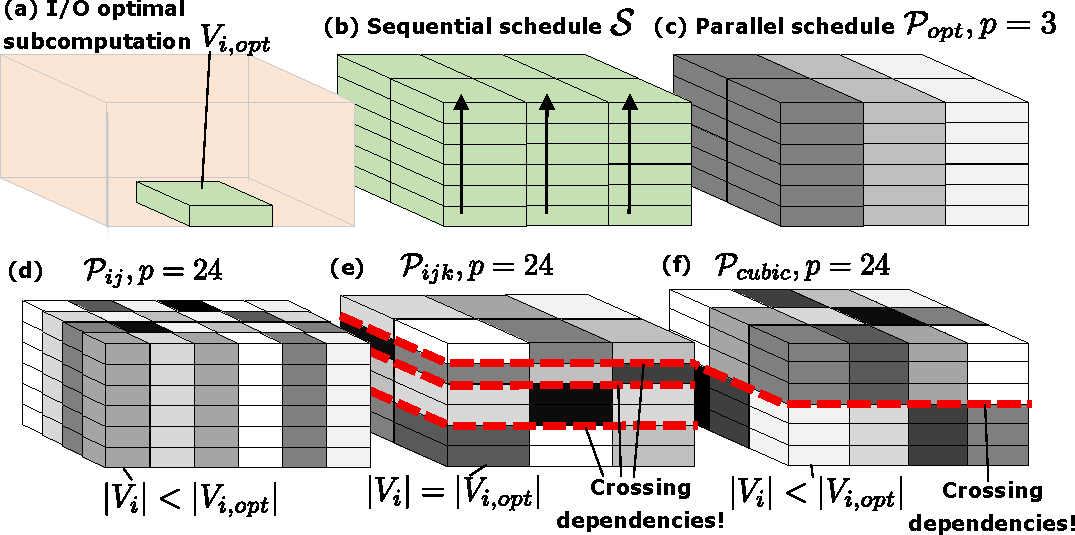
\includegraphics[width=\columnwidth]{figures/mmm_parallelization}
  \label{fig:mmmParallelization}
  \caption{Different parallelization schemes of matrix multiplication 
    arriving from the optimal sequential schedule. Up to six processes may 
    be 
    used optimally - above this limit we either increase I/O or 
    communication. 
    Shades of gray represent local domains of different processes. a) 
    Global 
    iteration domain (pink) and the optimal subset shape (green). b) Global 
    iteration space scheduling (arrows represent data dependencies). c) 
    Optimal 
    parallelization using $p=3$ processes. d-f) Suboptimal parallelization 
    using $p=24$ processes. From left to right, \textbf{par in ij}, 
    \textbf{par 
      in ijk} and \textbf{cubic}. Note the trade-off between I/O 
      (shrinkage of 
    local domain) and communication (dashed red lines showing 
    parallelization 
    and required communication in \textbf{k} dimension).} 
\end{figure}

We now analyze three possible parallelization strategies that either increase 
the I/O or the communication cost (or both) 
(Figure~\ref{fig:mmmParallelization}):

\begin{enumerate}
  \item \textbf{$\mathcal{P}ij$:} 
  The schedule is parallelized in dimensions \textbf{i} and 
  \textbf{j}. The process grid is $[m/a , n/a, 1]$, where $a = 
  \sqrt{\frac{mn}{p}}$.
  Because all dependencies are parallel to dimension \textbf{k}, no 
  communication is required $W(\mathcal{P}ij) = 0$, therefore 
  $\mathcal{P}ij$ is communication optimal. Because $a < \sqrt{S}$, the 
  corresponding sequential schedule $\mathcal{S}ij$ is not I/O optimal.
  \item \textbf{$\mathcal{P}ijk$} The schedule is parallelized in all 
  dimensions. The process grid is $[m/\sqrt{S} , n/\sqrt{S}, 
  mnk/(pS)]$.
   Each subcomputation's $V_i$ size is determined by 
  Equation~\ref{eq:seqSolution}: the sequential schedule is I/O optimal. The 
  parallelization in \textbf{k} dimension creates dependencies between local 
  domains, enforcing communication \\ $W(\mathcal{P}ijk) > 0$. 
  \item \textbf{$\mathcal{P}cubic$} The schedule is parallelized in all 
  dimensions. The process grid is $[m/a_c , n/a_c, 
  mnk/a_c]$, where $a_c = 
  \min\Big\{\big(\frac{mnk}{P}\big)^{1/3}, 
  \sqrt{\frac{S}{3}}\Big\}$. Because $a_c < \sqrt{S}$, the 
  corresponding sequential schedule $\mathcal{S}ij$ is not I/O optimal. 
  Also,  the 
  parallelization in \textbf{k} dimension creates dependencies between local 
  domains, enforcing communication $W(\mathcal{P}cubic) >\nobreak 0$. 
\end{enumerate}

\macb{Comparison with other algorithms:}

\begin{itemize}
  \item If $m = n$, $\mathcal{P}ij$ scheme is reduced to the
  classical 2D 
  decomposition (e.g., Cannon's algorithm~\cite{Cannon} or 
  SUMMA~\cite{summa}). 
  \item If $m = n = k$, $\mathcal{P}ijk$ reduces to 2.5D 
  decomposition~\cite{25d}.
  \item CARMA~\cite{CARMA} asymptotically reaches $\mathcal{P}cubic$
  scheme, 
  guaranteeing that 
  the longest dimension of a local cuboidal domain is at most two times 
  larger than the 
  smallest one.
\end{itemize}


%-------------------------Old version starts here
%\greg{------------------ Old version starts here -------------------}
%

%In this section we show how to derive a communication optimal parallel 
%schedule 
%from the
%results derived in ~\cref{sec:seqScheduling}. The explicit notion of reuse 
%effects
%\mac{reuse affects?} not only sequential \mac{the sequential} execution, as
%discussed above, but also parallel scheduling \mac{the parallel scheduling}, as
%it determines data dependencies \mac{It's unclear why only affecting data
%dependencies have impact on the parallel schedule}.  Intuitively, the schedule
%consists of $mnk/S$ elementary outer product calculations, arranged in
%$\sqrt{S} \times \sqrt{S} \times k$ "blocks" (Figure
%\ref{fig:mmmParallelization}). The number of dependency-free subsets in the
%optimal S-partition determines the maximum degree of parallelism up to which no
%additional \mac{What does it mean ``additional''?} communication between
%processes is performed. Above this threshold, further parallelization requires
%either parallelizing dependent subsets \mac{How? Sounds very vague}, causing
%additional communication between processes, or by shrinking the size of
%subsets, reducing the effective memory size \mac{Why? And what is effective
%memory size?}.
%
%\macb{Note: shared vs distributed memory model}. \mac{``Note:'' sounds bad, 
%like
%you're writing some report as homework. Too unstructured. A paper must like the
%inside of a watch, everything strutured for one goal. No some weirdo ``notes''}
%%
%In our work we only evaluate the total data volume transfered \mac{This now
%sounds like you start Evaluation, but it's the algorithmic part - very
%confusing. Why?} \mac{``evaluate the total volume'' - sounds very limiting. It
%is stressed even more by adding: ``only'' - you're essentially telling yourself
%that the analysis here is very limited :)} (both horizontally and vertically).
%For distributed \mac{a distributed} machine \mac{Actually, instead of machine,
%I'd write ``For distributed environments'' - sounds better}, we assume that a
%network is fully connected \mac{All such assumtions should be a part of a
%separate section where the whole distirbuted setting is summarized and
%explained}. We furthermore omit the analysis of congestion or latency
%\mac{Without any citation and a brief statement that it's a common approach, it
%sounds like it sucks}. With those assumptions, our results hold for both shared
%and distributed memory machine \mac{machines? or even better, environments?} -
%one can view the former as the latter with $p + 1$ processes, where the
%$(p+1)$st process mimics the shared memory \mac{Huh? Completely unclear, how
%mimic? No reference to support, bad.} - it holds the initial data and performs
%no work \mac{No work? What does it mean? Also, suddenly work-depth is brough
%up? Extremely confusing}. To translate the shared memory results to a
%distributed machine, one needs to subtract the cost of transferring the initial
%data layout \mac{But you just swaid above that it ``mimics'' and one can view
%one as the other on some more processes - and now it's about some additional
%subtraction? Extremely confusing}. We note however, that this accounts for up
%to additive factor $(mk + nk)/p$ of total communication volume. \mac{Anyone is
%lost again here. All these statements above must be clarified, ordered, and
%placed in a separate section on distributed settings}
%
%We now analyze three possible parallelization strategies that trade I/O for 
%communication optimality \mac{Unclear what this means - trade I/O - put more
%details, and make it more precise - for example, ``increase the number of
%I/O operations in exchange for...''} (Figure~\ref{fig:mmmParallelization}):
%
%\begin{enumerate}
%  \item \textbf{par. in ij dim:} 
%  Parallelization is only on the \textbf{ij} plane \mac{Unclear, write more
%  precisely wht this means that parallelism is on some plane - actually,
%  this should be just mentioned in the associated background section on MM
%  (that parallelizing a given plane is paralelizing the corresponding 
%loop(s))}, therefore there is no 
%  reuse 
%  (no data sent) \mac{Such connections between the I/O and distributed world 
%  like reuse --- data sent should be gathered and explicitly discussed 
%somewhere I guess...} 
%  between the processes (communication optimality). The local domain size is 
%  $[a \times a \times k]$, where $a = \sqrt{\frac{mn}{P}} < \sqrt{S}$  (I/O 
%  optimality \mac{the I/O optimality} is broken \mac{Cars can be broken, 
%broken optimality sounds bad}).
%  \item \textbf{par. in ijk dim:} The subset's size is 
%  constant determined by 
%  Equation~\ref{eq:seqSolution} (I/O optimality). The 
%  parallelization is done 
%  in all 
%  three dimensions \mac{You sometimes mention parallelism in the context of 
%planes, and
%  sotimes dimentions - confusing}. The reuse crossing domains of parallel 
%processes in 
%  \textbf{k} 
%  requires sending data between them (communication optimality 
%  is broken).
%  \item \textbf{cubic} 
%  the local domain size is 
%  $[a_c \times a_c \times a_c]$, where $a_c = 
%  \min\Big\{\big(\frac{mnk}{P}\big)^{1/3}, 
%  \sqrt{\frac{S}{3}}\Big\}$ (both I/O and communication 
%  optimality is broken \mac{broken again}).
%\end{enumerate}
%

\subsection{Data Movement Optimal Parallel Schedule}
\label{sec:parScheduling}
Observe that none of those schedules is optimal in the whole range of 
parameters.
As discussed in ~\cref{sec:seqScheduling}, in sequential 
scheduling, 
intermediate results of C are not stored to the memory - they are 
consumed 
(reused) immediately by the next sequential step. Only the final 
result of C in 
local domain is sent. Therefore, the optimal parallel schedule 
$\mathcal{P}_{Copt}$
minimizes the 
communication, that is, sum of the inputs' sizes plus the output 
size, under 
the sequential I/O constraint on subcomputations $\forall_{V_i \in 
\mathcal{P}_{Copt}} |\mathcal{I}_i| \le S \land |\mathcal{O}_i| \le S$.

The local domain $\mathcal{D}_j$ is a cuboid of size $[a \times a \times b]$. 
The optimization problem of finding $\mathcal{P}_{Copt}$
using the 
computational intensity (~\cref{sec:compIntensity}) can be 
formulated as 
follows:
\begin{multline}
\label{eq:tileEq}
\\
\text{maximize } \rho = \frac{a^2b}{ab + ab + a^2}\\
\text{subject to: } \\
a + a + a^2 \le S \text{ (I/O constraint)} \\
a^2b = \frac{mnk}{p} \text{ (load balance constraint)} \\ 
\end{multline}
where $p$ is the number of processes. The inequality constraint $2a + 
a^2 \le 
S$ is tight (binding) for $p \ge \frac{mnk}{S^{3/2}}$. Therefore, the solution 
to this problem (using the 
approximation~\ref{eq:approx}):

\begin{multline}
\\
a = \min\Big\{\sqrt{S}, \Big(\frac{mnk}{p}\Big)^{1/3} \Big\}\\
b = \max\Big\{\frac{mnk}{pS}, \Big(\frac{mnk}{p}\Big)^{1/3} \Big\}\\
\label{eq:optTileShape}
%\end{cases}\\
\end{multline}
\\

This can be intuitively interpreted geometrically as follows: if we 
imagine the 
optimal local domain "growing" with decreasing number of processes, 
then it is 
cubic until it is still "small enough" (its side is smaller than 
$\sqrt{S}$). 
After that point, its face in \textbf{ij} plane stays constant 
$\sqrt{S} \times 
\sqrt{S}$ and it "grows" 
only in the \textbf{k} dimension. This schedule effectively switches 
from $\mathcal{P}ijk$ to $\mathcal{P}cubic$ once there is enough 
memory ($S \ge \big(\frac{mnk}{p}\big)^{2/3}$).

\begin{lma}
  \label{lma:parSchedule}
  Parallel schedule $\mathcal{P}_{Copt} = \{\mathcal{D}_j\}$ composed of $p$ 
  local domains $\mathcal{D}_j$ of size 
  determined by Equation~\ref{eq:optTileShape} is asymptotically 
  communication optimal, that is, the communication volume is minimal across 
  all parallel schedules $\mathcal{P}$ with $p$ processes.
\end{lma}

\begin{proof}
The communication cost $W$ of each local domain $\mathcal{D} \in 
\mathcal{P}_{Copt}$ is the sum of communications of all subcomputations $V_i 
\in \mathcal{D}$. Each subcomputation $V_i$ requires $2a$ elements to be 
communicated (~\cref{sec:seqOptimality}). The number of subcomputations is 
$|\mathcal{D}| = b$. Furthermore, the last subcomputation $V_b$ must 
communicate $a^2$ outputs. Therefore, the total communication cost $W$ 
is: 
t%he sum of communications of all processes:


$$W = \max\Big\{\frac{2mnk}{\sqrt{S}} + 
S, 3\Big(\frac{mnk}{p}\Big)^{2/3}  \Big\}$$

This schedule is asymptotically communication optimal, as it reaches both 
memory-dependent and 
memory-independent lower bounds~\cite{memIndependentBound}.
\end{proof}

\subsection{Discussion}

\subsubsection{I/O-Latency Trade-off}
As showed in~\cref{sec:parScheduling}, the local domain $\mathcal{D}$ of the 
I/O optimal 
schedule $\mathcal{P}$ is a cuboid of size $[a \times a \times b]$, where $a, 
b$ are given by Equation~\ref{eq:optTileShape}. The I/O cost of each  
$\mathcal{D}$ is $2ab$ (size of the inputs) plus $a^2$ (output). 
 The corresponding sequential 
schedule $\mathcal{S}$ is a sequence of $b$ outer products of vectors of length 
$a$. Denote the size of the required inputs in each step by $I_{step} = 2a$. 
However, this corresponds to $b$ steps of communication ($C_L = b$).

The number of steps (latency) is equal to the communication volume divided by 
the volume per step $C_L = W/I_{step}$. To reduce the latency, one 
either have to decrease $W$ or increase $I_{step}$, under the memory 
constraint that $I_{step} + a^2 \le S$ (otherwise we cannot fit the inputs and 
the outputs in the memory). Express $I_{step} = a \cdot h$, where $h$ is the 
number of sequential subcomputations $V_i$ we merge in one communication. We 
can now express the I/O-latency trade-off:

\begin{multline}
\\
W = 2ab + a^2 \\
C_L = \frac{b}{h} \\
a^2 + 2ah \le S \text{(I/O constraint)} \\
a^2b = \frac{mnk}{p} \text{(load balance constraint)} \\
\end{multline}
Solving this problem, we have $W = \frac{2mnk}{pa} + a^2$ and $C_L 
= 
\frac{mnk}{pa(S-a^2)}$, 
where $a \le \sqrt{S}$. Increasing $a$ we \emph{reduce} I/O cost 
$W$ and \emph{increase} latency cost $C_L$. For minimal value of 
$W$ (Lemma~\ref{lma:parSchedule}),  $C_L = \max\{\frac{2a^2}{S - 
a^2}\}$, where $a = \min\{\sqrt{S}, (mnk/p)^{1/3} \}$. Based on our 
experiments, we observe that the I/O cost is vastly greater than the 
latency cost, therefore our schedule by default minimizes $W$ and uses 
extra memory (if any) to reduce $C_L$. However, we leave that as a tunable 
parameter dependent on the hardware parameters.

\subsubsection{Parallel efficiency} 
We now proceed to analyze the 
communication's 
\emph{parallel efficiency} of all parallelization schemes. We define it as a 
ratio between  
the total data movement required by the sequential processor (Theorem 
\ref{thm:seqlowbounds}) and sum of data movements performed by all 
parallel
processes. More 
formally, if $Q(p,S)$ is the data movement cost per process of the 
algorithm 
using $p$ 
processes, each of local fast memory size $S$, then the parallel 
efficiency 
metric for communication is defined as $E(p,S) = 
\frac{Q(1,S)}{pQ(p,S)}$.

In the proof of Lemma~\ref{lma:parSchedule} we derive $pQ(p,S)$ for 
$\mathcal{P}Copt$. Using the same technique, we obtain $pQ(p,S)$ for the 
remaining schedules $\mathcal{P}ij$, $\mathcal{P}ijk$, and $\mathcal{P}cubic$.
The results of our analysis is shown in Table \ref{tab:mmmEfficiency} 
and 
Figure \ref{fig:mmmScaling}.


\begin{table*}[t]
  \begin{tabular}{lllll}
    \toprule
    range & metric & par in \textbf{ij} dim & par. in 
    \textbf{ijk} dim & 
    cubic \\
    \midrule 
    %
    \multirow{3}{*}{$p \le \frac{mn}{S}$}
    %
    & loc. dom. & $[\sqrt{S} \times \sqrt{S} \times k]$ & 
    $[\sqrt{S} 
    \times \sqrt{S} \times k]$ & $\Big[\sqrt{\frac{S}{3}} \times 
    \sqrt{\frac{S}{3}} \times \sqrt{\frac{S}{3}}\Big]$ \\
    \cline{2-5}
    %
    & $pQ(p,S)$ & 
    $\frac{2mnk}{\sqrt{S}} + mn$ & 
    $\frac{2mnk}{\sqrt{S}} + mn$ & 
    $\frac{3\sqrt{3}mnk}{\sqrt{S}}$ \\
    \cline{2-5}
    %
    & $E(p,S)$ & 1 & 1 &   $\frac{2K + 
    \sqrt{S}}{3\sqrt{3}k}$ \\
    \midrule 
    %
    \multirow{3}{*}{
      \begin{tabular}{l}
        $\frac{mn}{S} < p$ \\
        $p \le \Big(\frac{3}{S}\Big)^{3/2}mnk$
      \end{tabular}     
    }
    % 
    & loc. dom. & $\Big[\sqrt{\frac{mn}{p}} \times 
    \sqrt{\frac{mn}{p}} 
    \times k\Big]$ & $\Big[\sqrt{S} 
    \times \sqrt{S} \times \frac{mnk}{Sp}\Big]$ & 
    $\Big[\sqrt{\frac{S}{3}} 
    \times 
    \sqrt{\frac{S}{3}} \times \sqrt{\frac{S}{3}}\Big]$ \\
    \cline{2-5}
    %
    & $pQ(p,S)$ & $2K 
    \sqrt{pmn} + mn$ & 
    $\frac{2mnk}{\sqrt{S}} + pS$ & 
    $\frac{3\sqrt{3}mnk}{\sqrt{S}}$ 
    \\
    \cline{2-5}
    %
    & $E(p,S)$ & $\frac{mnk(\frac{2}{\sqrt{S}} + 
    \frac{1}{k})}{2K\sqrt{MNp} 
    + mn}$ & $\frac{2mnk(1 + \frac{\sqrt{S}}{2K})}{2mnk + 
    S^{3/2}p}$ &   
    $\frac{2K + 
      \sqrt{S}}{3\sqrt{3}k}$ \\
    \midrule \\
    %
    \multirow{3}{*}{$p > \Big(\frac{3}{S}\Big)^{3/2}mnk$}
    %
    & loc. dom. & $\Big[\sqrt{\frac{mn}{p}} \times 
    \sqrt{\frac{mn}{p}} 
    \times k\Big]$ & $\Big[\sqrt{S} 
    \times \sqrt{S} \times \frac{mnk}{Sp}\Big]$ & 
    \begin{tabular}{l}
$\Big[a 
\times 
a \times 
a\Big]$ \\
$a = \big(\frac{mnk}{p}\big)^{1/3}$
    \end{tabular} 
  \\
  \cline{2-5}
    %
    & $pQ(p,S)$ & $2K 
    \sqrt{pmn} + mn$ & 
    $\frac{2mnk}{\sqrt{S}} + pS$ & 
    $3p\big(\frac{mnk}{p}\big)^{2/3}$ 
    \\
    \cline{2-5}
    %
    & $E(p,S)$ & $\frac{mnk(\frac{2}{\sqrt{S}} + 
    \frac{1}{k})}{2K\sqrt{MNp} 
      + mn}$ & $\frac{2mnk(1 + \frac{\sqrt{S}}{2K})}{2mnk + 
      S^{3/2}p}$ &   
    $\frac{2mnk(1 + 
    \frac{\sqrt{S}}{2K})}{3p^{1/3}\sqrt{S}(mnk)^{2/3}}$ \\
  \end{tabular}
  \caption{Total communication volume of MMM and its parallel 
  efficiency of 
  the 
  different parallelization schemes. We assume that all the 
  respective local 
  domain sizes divide the global matrix sizes evenly (e.g., for 
  cubic domain 
  in range $p \le mn/S$, we assume that $\sqrt{S/3} = a_1M = a_2N = 
  a_3K$ for 
  $a_1, a_2, a_3 \in \mathbb{N}$). The optimal schedule 
  (\cref{sec:parScheduling}) switches from \textbf{par. in ijk} to 
  \textbf{cubic} when $p \ge \frac{mnk}{S^{3/2}}$.}
  \label{tab:mmmEfficiency}
\end{table*}


 \begin{figure*}[t]
     \centering
   %
   \hspace{-1cm}
   \subfloat["flat" matrices]{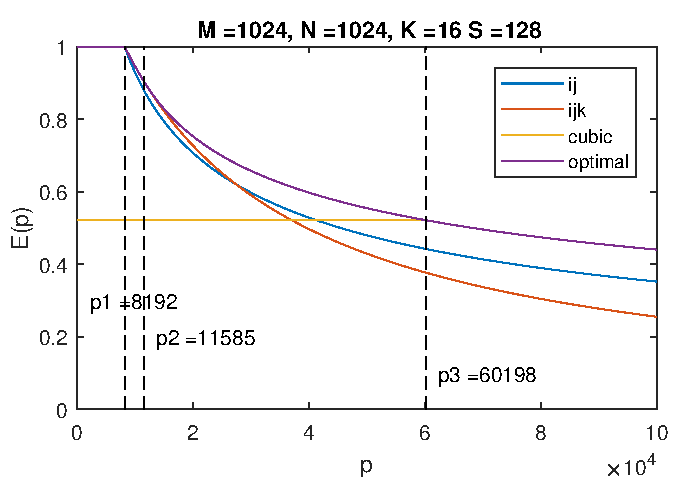
\includegraphics[width=0.33\textwidth]
     {figures/efficiencyPlot11}\label{fig:effic1}}
   %
 %\hfill
   %
   \subfloat[square matrices, small 
   $S$]{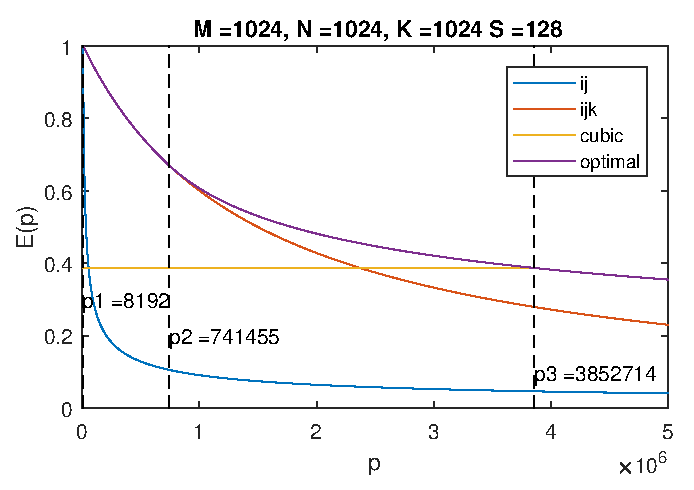
\includegraphics[width=0.33\textwidth]
     {figures/efficiencyPlot12}\label{fig:effic2}}
   %
  %\hfill
   %
   \subfloat[square matrices, large 
   $S$]{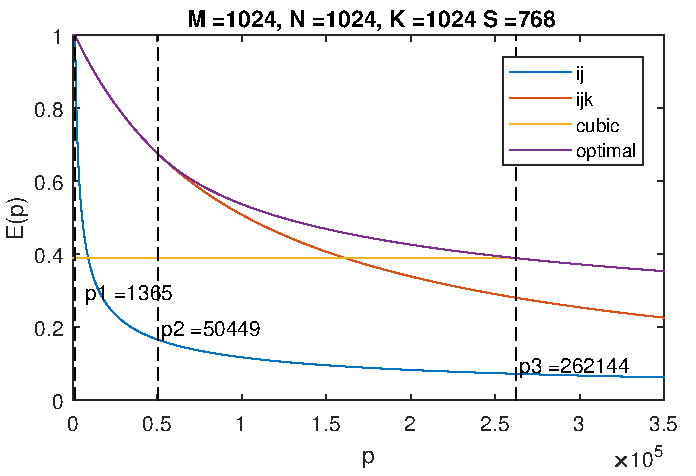
\includegraphics[width=0.33\textwidth]
     {figures/efficiencyPlot13}\label{fig:effic3}}
   %
   \hspace*{-1.5cm}
   \caption{Parallel 
   efficiency 
   of different parallelization schemes. Three vertical dashed lines 
   correspond to 
     thresholds 
     $p1 = mn/S$, $p2 = mnk/S^{3/2}$ and $p3 = 
     (\frac{3}{S})^{3/2}mnk$ (Table \ref{tab:mmmEfficiency}). Note 
     that for cases (b) and (c), increasing memory $S$ six times 
     reduces the number of processes required to fully saturate it 
     drops from $p2=741455$ to $p2=50449$. }
   \label{fig:mmmScaling}
 \end{figure*}

\section{Implementation}
\label{sec:implementation}
In this Section we discuss various implementation insights that further 
increase the performance of our code. To leverage the RDMA mechanisms of 
current high-speed network interfaces, we use MPI one-sided 
interface(~\cref{sec:rdma}). We also use an block-cyclic data 
layout(~\cref{sec:datalayout}), grid-fitting 
technique(~\cref{sec:decompArbitrary}) and an optimized binary broadcast 
tree using static information about
the communication pattern(~\cref{sec:commPattern}) together with the buffer 
swapping(~\cref{sec:bufferReuse}). For the local matrix operations, we use 
BLAS routines. Together, those optimizations account 
for XX total runtime 
reduction. 

\subsection{Blocked Data Layout}
\label{sec:datalayout}



\subsection{Fitting Process Grid to Problem Size}
\label{sec:decompArbitrary}
\begin{figure}[!tbp]
	\centering
	%
	\subfloat[$1 \times 3 \times 15$ 
	grid]{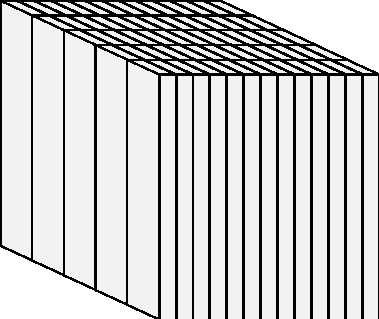
\includegraphics[width=0.18\textwidth]
		{figures/proc_decomp_problem_bad}\label{fig:decomp_left}}
	%
	\hfill
	%
	\subfloat[$4 \times 4 \times 4$ grid with one idle 
	process]{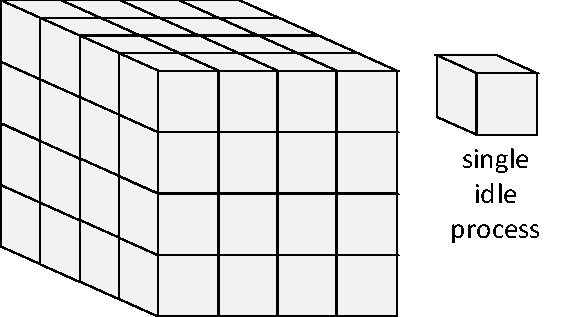
\includegraphics[width=0.27\textwidth]
		{figures/proc_decomp_problem_good}\label{fig:decomp_right}}
	%
	\caption{Process decomposition for square matrices and 65 
		processes. To utilize all resources, the local domain is 
		drastically stretched (a). Dropping one 
		process results in a symmetric grid (b) that 
		increases the computation per process only by 1\%, but reduces 
		the communication by 36\%.}
	\label{fig:decompProblem}
\end{figure}
Throughout the paper, we assume all operations required to 
assess the decomposition (divisions, roots, powers) result in natural 
numbers. We note that in practice it is rarely the case - e.g., the 
$[8704 \times 8704 \times 933888]$ domain, emerging from an exemplary 
water molecule simulation~\cite{joost}, when launched on the whole 
Piz Daint supercomputer with 1813 nodes, cannot be equally divided. 
Moreover, the memory size per 
node (64~GiB DDR, 90~MiB L3 cache) does not give the integer solution 
for the Equation~\ref{eq:seqSolution} ($a = \sqrt{S+1} -1$) for the 
local domain size. One may use the straightforward approach to take  
the floor and ceiling
functions for non-natural numbers, but this may result in suboptimal 
results, as we demonstrate in the following example.

Assume that we multiply two square matrices with 65 
processes (Figure~\ref{fig:decompProblem}). The only integer factors 
of 65 are 1, 5 and 13. Therefore, to 
utilize all the resources, the processes must be arranged in a $[13 
\times 5 \times 1]$ grid (up to a permutation). On the other hand, if 
we decide \emph{not to utilize all resources} 
and drop one process, then we can arrange remaining 64 in a $[4 
\times 4 \times 4]$ grid. Such arrangement \emph{trades communication 
	for computation:} it increases the number of arithmetic operations 
per process by 1\%, while decreasing the communication volume per 
process by 36\%. However, because the dense MMM is compute bound, the 
decision which arrangement is better is not obvious.
% In this extreme example the trade-off is clearly visible, but 
%In most real life scenarios it is a non-trivial decision 
%and depends on the computation and communication performance of a 
%machine. 
In most real life scenarios this trade-off may vary and the optimal 
decomposition depends on the computation and communication 
performance 
of a 
machine. 


%This gives $2.15\cdot10^9$ arithmetic operations 
%(only 1\% increase) and $3\cdot10^6$ elements communicated (36\% 
%decrease).
%This results in 
%$2.12\cdot10^9$ arithmetic operations and approx. $5\cdot10^6$ 
%elements communicated per process.

The existing algorithms either cannot handle such case (CARMA), 
require a user to manually specify the decomposition (ScaLAPACK), or 
simply discard the "non-fitting" processes using floor functions 
(Cyclops). Our algorithm balances this computation-communication 
trade-off by "stretching" the local domain size 
derived in ~\cref{sec:parScheduling} to fit the global 
domain by adjusting its width, height and length. The range of this 
tuning (how far is the shape of the local domain from the optimal, 
increasing communication but utilizing more resources) 
depends on the hardware specification of the 
machine (peak FLOP/s, memory and network bandwidth) and it is a
tunable parameter. For our 
experiments on Piz Daint we chose the maximal ratio between the 
optimal and applied size to be ??, accounting for up to ?? speedup 
compared to a straightforward (applying floor and ceiling functions) 
decomposition.

\subsection{Communication Pattern}
\label{sec:commPattern}
As shown in Algorithm~\ref{alg:comm}, COMM executes $\frac{2ab}{S - a^2}$ 
steps. In each step, each process receives $\frac{S - a^2}{2a}$ elements of A 
and 
B. Therefore, the inputs has are broadcast among the \textbf{i} and \textbf{j} 
dimensions of the process grid. After the last step, the partial results of C 
are reduced among the \textbf{k} dimension. The communication pattern is 
therefore similar to ScaLAPACK or Cyclops.

To accelerate the collective communication, we implement our own binary 
broadcast 
tree, taking advantage of a static data layout, process grid and communication 
pattern.
 Knowing the initial data 
layout(~\cref{sec:datalayout}) and the process 
grid(~\cref{sec:decompArbitrary}), we craft the binary reduction tree 
in all three dimensions \textbf{i}, \textbf{j} and \textbf{k} such that a 
distance in the grid between communicating processes is minimized. 

Given a $[g_M, g_N, g_K]$ process grid, in each dimension we organize processes 
in a balanced binary tree with $g_i$ leaves ($i \in \{m,n,k\}$). The 
communication 
(either distributing inputs A and B, or reducing output C) is performed in 
$\left \lceil{log_2(g_i)} \right \rceil$ steps, sending data of size $2^(s-1) 
D$, where $s$ is the step 
number and $D$ is the local size of data to be distributed.

\subsection{One-Sided and Two-Sided Communication}
\label{sec:rdma}
To reduce the latency \greg{cite something?} we implemented the communication 
using MPI one-sided~\cite{mpi3-rma-overview}. This interface utilizes the 
underlying features of RDMA (Remote Direct Memory Access) mechanism, bypassing 
the OS on the receiver side and providing zero-copy communication (data sent is 
not buffered in a temporary address, instead, it is written directly to its 
destination).

Due to the static nature of the algorithm, all communication windows are 
pre-allocated using MPI\_Win\_Allocate with the size of maximum message in the 
broadcast tree $2^(s-1) D$ (~\cref{sec:commPattern}). Communication in each 
step is performed using MPI\_Put with passive synchronization (MPI\_Lock / 
MPI\_Unlock).

For compatibility reasons, as well as for the performance comparison, we also 
implemented a communication back-end using MPI two-sided (message passing 
abstraction). In our tests on Piz Daint, we observed that the two-sided version 
was XX faster/slower than the one-sided.


\subsection{Local buffer reuse}
\label{sec:bufferReuse}
The binary broadcast tree pattern of our communication is a generalization of 
the recursive structure CARMA algorithm. However, CARMA in each step of the 
recursion dynamically allocates new buffers of increasing size to match the 
message sizes $2^{s-1} D$, causing additional runtime overhead.

To alleviate this problem, we use our static knowledge and pre-allocate a 
single buffer per matrix A, B and C of the maximum size of the message $ab/t$, 
where $t = \frac{2ab}{S - a^2}$ is the number of steps in COMM 
(Algorithm~\ref{alg:comm}). Then, in each level $s$ of the communication tree, 
we  move the pointer in the receive buffer by $2^{s-1} D$ elements.

%We offer two versions of the algorithm: an \emph{asynchronous} 
%version using the one-sided communication backend and a 
%\emph{synchronous} version using the two-sided communication. The 
%choise of the version to be used can be made at the runtime of the 
%algorithm. In the asynchronous version, each rank has a read-only 
%buffer that holds the initial data and the data from this buffer can 
%be fetched by any processor at any time without any synchronization 
%between processors. This allows a natural separation of the logic 
%behind the initial data layout and the computation: what a processor 
%computes as the output might be independent of what data this 
%processor initially owns, thus allowing an overlap of communication 
%and computation. The drawback of this approach is that a processor 
%cannot use this initial buffer, they are read-only and they only 
%serve to allow the access to this data for any process that might 
%need it. In the two-sided version, the communication happens in 
%synchronously: whenever a processor has to compute some subproblem, 
%it will first collect all the necessary input data and then perform 
%the computation. Here, instead of always exchanging just the content 
%of the \emph{initial}, read-only buffers (as in the one-sided 
%version), the processors exchange the content of the current, 
%\emph{working} buffers, which they also actively use. For this 
%reason, we want to avoid the need of local data reshuffling in these 
%\emph{working} buffers which might be needed after the communication. 
%This can be achieved by carefully corellating the initial data layout 
%with the order of the data exchanges throughout the algorithm, which 
%is explained in the next section. 
%
%\greg{We use two buffers instead of $\log P$}

\section{Evaluation}
\label{sec:evaluation}

We evaluate COMM against other state-of-the-art implementations with various 
combinations of matrix dimensions and memory requirements. These scenarios 
include both synthetic square matrices, in which all algorithms achieve their 
peak performance, as well as real-world "tall-and-skinny" cases with uneven 
number of available processes. 
 
%\mac{My papers, for example, RMA Locks or Push Pull, or Slim NoC,
%contain good Evaluation sections, I'd suggest checking them in case
%of some doubts}

\macb{Comparison Targets}
%
As a comparison, we use a widely used ScaLAPACK library (commit number 3287fdd 
on May 17, 2018), as well 
as Cyclops Tensor Framework (commit number 6aaf037 on February 16, 2018) and 
the original CARMA implementation (commit number 7589212 on July 19, 2013).

%\macb{Datasets}
%%
%\mac{What concrete datasets are used?}
\macb{Matrix Dimensions and Number of Processes}
We use both square ($m = n = k$) and "skinny" ($m = n << k$) matrices. Due to 
the space constraints, we skip the "flat" (e.g., $m << n = k$) case and limit 
ourselves to these two extreme cases. The matrix dimensions and number of 
processes are (1) powers of 
two $m = 2^{r_1}, n = 2^{r_2}, m = 2^{r_3}$, (2) determined by the real-life 
simulations or hardware architecture (available nodes on a computer), (3) 
chosen from a random distribution. 
For our "skinny" matrix, we consider the problem of 
water 
molecules interaction in the DFT
simulation\cite{joost}. There, to simulate $w$ molecules, the sizes 
of the 
matrices are $m=n=136w$ and $k = 228w^2$. We use $w=64$ as in the 
original paper, yielding $m=n=8704, k = 933888$.

\macb{Selection of Benchmarks}
%
We perform both strong scaling and \emph{adjusted size} experiments. 
The \emph{adjusted size} scenario fixes the input size per process 
($\frac{pS}{I}, I = mn + mk + nk$), as opposed to the work per 
process ($\frac{mnk}{p} \ne const$). We evaluate two cases: (1) "just enough 
memory" ($\frac{pS}{I} = 1$), and (2) "extra memory"  ($\frac{pS}{I} = 
p^{1/3}$).
%
%\mac{Instead of this list, I'd suggest use a block of text (list in text)
%like in my Push Pull paper or in RMA Locks paper}
%%
%We chose our experiments to cover the whole spectrum of possible use 
%cases. We 
%compare
%\begin{itemize}
%  \item square ($m=n=k$) vs "skinny" ($m=n << k$) matrices,
%  \item different memory requirements: just enough memory to fit 
%  the inputs 
%  ($S = (mk + nk)/p$) vs enough memory for $p^{1/3}$ redundant 
%  copies of data,
%  \item weak vs strong scaling,
%  \item parameter values that are powers of two vs randomly chosen 
%  vs 
%  determined by real-life problem definition.
%\end{itemize}
%
%For our "skinny" matrix, as a use case we evaluate the problem of 
%water 
%molecules interaction in the DFT
%simulation\cite{joost}. There, to simulate $w$ molecules, the sizes 
%of the 
%matrices are $m=n=136w$ and $k = 228w^2$. We use $w=64$ as in the 
%original paper, yielding $m=n=8704, k = 933888$.
%
%\macb{Varied Parameters}
%%
%\mac{Are there any additional important parameters to be explicitly described?}

\macb{Programming Models}
%
As stated in (~\cref{sec:rdma}), we use both RMA and Message Passing models. 
CARMA, ScaLAPACK and CTF ?? use MPI two-sided (Message Passing).

\macb{Experimentation Methodology}
%
For each combination of parameters, we perform 20 runs. As all the algorithms 
use BLAS routines for local matrix computations, we discard the first run due 
to the BLAS setup overhead. We report median and 95\% confidence intervals of 
the runtime.
%\mac{How is data gathered? What is considered? Info on statistical measures,
%confidence intervals, other statistical info}

\macb{Experimental Setup and Architectures}
%
We run our experiments on CSCS Piz Daint - Cray supercomputer equipped with
5320 XC50 heterogeneous nodes with NVIDIA Tesla P100 and 1813 XC40 nodes with
dual-socket Intel Xeon E5-2695 v4 processors (3.30 GHz,45 MiB L3 shared cache, 
64 GiB DDR3 RAM),
interconnected with Cray Aries network.

\macb{Infrastructure and Implementation Details}
%
All implementations were compiled using the gcc 5.3.0 compiler. We use 
Cray-MPICH 3.1 implementation of MPI. The intra-node parallelism is handled 
internally by the MKL BLAS version 2017.4.196. 
%\mac{Any information about, for example, version of MPI used, and/or
%things like PAPI, OpenMP? Also versions of used compilers, etc.}

\section{Results}
\label{sec:results}
\greg{No results yet. Waiting for Marko}



%\begin{multline}
%\\
%G = (V,E) \\
%|V| = n \\
%|E| = m \\
%p partitions \\
%\forall_{i = 1..p} P_i \in V \\
%\bigcup_{i = 1..p} P_i = V \\
%\bigcap_{i = 1..p} P_i = \emptyset \\
%\forall_{i = 1..p} BE_i \in E = \{(u,v) : u \in P_i \land v \notin P_i\} \\
%\forall_{i = 1..p} BV_i \in V = \{u : (u,v) \in BE_i\} \\
%pl_i(u,v) = \{e \in E \cap (P_i \times P_i) : \text{edges connect u and v} \} 
%- 
%\text{local path between u and v} \\
%pr_i(u,v) = \{e \notin E \cap (P_i \times P_i) : \text{edges connect u and v} 
%\} - \text{remote path between u and v} \\
%\end{multline}
%\begin{enumerate}
%  \item For each $P_i$:
%\end{enumerate}

\section{Related work}

Data movement minimization essentially may be divided into two aspects: across 
memory hierarchy (vertical, also called I/O minimization) and between parallel 
processes (horizontal, also called communication minimization). Even though 
they are two sides of the same coin, in literature they are often treated as 
separate topics. In our work we combine two together, that is, analyzing 
trade-offs between 
communication optimal (distributed memory) and I/O optimal schedule 
(shared memory). We observe that even though algorithms of the second class 
tend to be problem size independent, distributed memory algorithms fix the 
domain sizes based on the even process grid (as discussed in Introduction - 
"top-down" vs "bottom-up" approach).

\subsection{General I/O Lower Bounds}
I/O optimization techniques date back to work by 
Sethi~\cite{completeRegisterProblems}, where he used one color pebble game to 
model minimum number of registers required to perform a computation. It has 
been proven by Gilbert et.al~\cite{pebblegameregister} that this problem is 
P-SPACE complete. Despite the complexity, much work based on pebble game 
abstraction. Paul and Tarjan~~\cite{pebbleTradeoffs} studied time-space 
tradeoffs in pebble games. Dymond and Tompa~\cite{dymond2playerpebblegame} 
developed a 
two-player game to study parallel speedups. Most notably, Hong and 
Kung~\cite{redblue} introduced red-blue pebble game, on which our work is 
based. Elango et al.~\cite{redbluewhite} extended this work to red-blue-white 
game and Liu and Terman~\cite{redblueHard} proved that it is also P-SPACE 
complete. Chan~\cite{justApebbleGame} studied different variants of pebble 
games in context of memory space and parallel time. Aggarwal and 
Vitter~\cite{externalMem}
introduced a two-memory machine that models a blocked access and latency in an
external storage. Large et al.~\cite{parallelExMem} extended this model to a 
parallel machine. Solomonik et al.~\cite{edgarTradeoff} combined the 
communication, synchronization and computation in their general cost model and 
applied 
it to several linear algebra algorithms.

\subsection{Shared Memory Optimizations}
Memory optimization for linear algebra includes such techniques as loop tiling 
and skewing~\cite{tiling}, interchanging and reversal~\cite{tiling2}. For 
programs with multiple loop nests, Kennedy and McKinley~\cite{loopFusion} 
showed various techniques for loop fusion and proved that in general this 
problem is NP-hard. Later, 
Darte~\cite{loopFusionComplexity} identified cases when this problem has 
polynomial complexity.

Toledo~\cite{IOsurvey} in his survey on Out-Of-Core (OOC) algorithms analyzed 
various I/O minimizing techniques for dense and sparse matrices, like 
multiplication, factorization, or iterative methods. 
Mohanty~\cite{MohantyThesis} in his thesis optimized various OOC algorithms for 
QR, QZ decompositions and eigenvalue computation, expressing them with MMM 
kernels. Irony et 
al.~\cite{IronyMMM} proved the I/O lower bound of classical MMM on a parallel 
machine. Ballard et al.~\cite{strassenBounds} proved analogous results for 
Strassen's algorithm. This analysis was extended by Scott et 
al.~\cite{generalStrassenBounds} to a general class of Strassen-like algorithms.

Although we consider only dense matrices, there is an extensive literature on 
sparse matrix I/O optimizations. Bender et al.~\cite{SpMVIO} extended 
Aggarwal's external memory model~\cite{externalMem} and showed I/O complexity 
of sparse matrix-vector (SpMV) multiplication under various data layouts. 
Greiner~\cite{SpEverything} extended those results and provided parallel I/O 
complexities of other sparse computations, like bilinear forms or sparse-sparse 
and sparse-dense matrix multiplications.


\subsection{Distributed Memory Optimizations}
Parallel algorithms for matrix multiplication dates back to the work of 
Cannon~\cite{Cannon}, which has been analyzed and extended many times, e.g, 
~\cite{MManalysis}~\cite{generalCannon}. In the presence of extra memory, 
Aggarwal et al.~\cite{summa3d} included parallelization in the third dimension. 
Solomink and Demmel~\cite{25d} extended this scheme to arbitrary range of 
available memory, effectively interpolating between Cannon's 2D and Agarwal's 
3D scheme. Recursive, cache-oblivious MM algorithm was introduced by Blumofe 
et al.~\cite{recursiveMM} and extended to rectangular matrices by Frigo et 
al.~\cite{recursiveRectangularMM}. Demmel el al.~\cite{CARMA} showed that their 
recursive CARMA algorithm achieves asymptotic complexity for all matrix and 
memory sizes. 

\section{Conclusions}
In our work we show that starting from the sequential I/O optimality we achieve 
optimal parallel communication optimality for any combination of input 
parameters. We introduce a new proof of sequential and parallel matrix 
multiplication data movement complexity, giving tight leading constants. We 
advocate that asymptotic analysis alone is not enough to draw conclusions on 
the real-life performance of the algorithms. We 
compare (name of our algorithm here) with existing state-of-the-art schedules, 
showing the 
superiority of the former both in terms of theoretical analysis and achieved 
performance.

%\greg{
%  TODO: 
%  \begin{enumerate}
%    \item BSP model?
%  \end{enumerate}
%}
%
%\section{Bibliography}

%% Bibliography style
%\bibliographystyle{ACM-Reference-Format}

\bibliographystyle{ACM-Reference-Format}
\bibliography{mmm-ppopp}

\appendix


\section{Tighter General I/O Lower Bounds}
\label{sec:background}

To prove the I/O optimality of COMM, we start with deriving a new constructive 
proof 
of
the MMM sequential I/O lower bound. We refine the existing asymptotic bound $Q 
= \Omega(\frac{mnk}{\sqrt{S}})$ by Hong and
Kung~\cite{redblue}, and $Q \ge \frac{2mnk}{\sqrt{S}} - 2S$ by Smith and van de 
Gein~\cite{tightMMM} and derive a new bound $Q \ge \frac{2mnk}{\sqrt{S}}$. 
Although we note that this is just an additive improvement over the latter 
result, we use the same mathematical machinery to generate an I/O optimal 
\emph{parallel} schedule. This machinery extends the methods used by Hong and
Kung,  heavily relying on the \emph{red-blue
	pebble game} and the \emph{$S$-partition abstraction}. 
%
%\mac{For the whole document: do NOT use tabs, use double spaces instead.}
%
%This section discusses the \mac{used} sequential and parallel machine models,
%as well as \mac{the} necessary concepts of pebble games in the context of
%\mac{``in the context of'' --> ``and'' (simpler)} I/O optimality.
%
%\mac{As this whole stuff is very complex and spans multiple domains, I think
%it may be a good idea to provide, at the beginning of each subsection, a
%sentence describing WHY we care, linking to MM (when describing I/O), linking
%to I/O (when describing MM), etc.}
%
%% We modify Hong and Kung's lemma (inequality \ref{eq:redbluebound}) %to prove
%the tighter lower bound (inequality \ref{eq:reusebound}), which %explicitly
%expresses \emph{data reuse} - that is, a subset of data used by %some part of
%computation that is used by the following part and is kept in the %fast
%memory. In the context of matrix multiplication, the original one takes %an
%upper bound of the data reuse and corresponds to case b) in Figure
%%\ref{fig:mmmreuse}. Our result maximizes the achievable reuse, showed in case
%%c) in Figure \ref{fig:mmmreuse}.  Readers not interested in deriving Lemma
%%\ref{eq:reusebound} may proceed directly to Section \ref{sec:seqOptimality}.
%%The most important symbols are gathered in Table~\ref{tab:symbols}.
%
%%\mac{This whole paragraph is extremely confusing, let's chat.}


%
%\subsection{Sequential Machine Model}
%\label{sec:seq-model}
%
%\mac{Repeat briefly why we care and how it links to MM}
%%
%We use the sequential computation model from Hong and Kung~\cite{redblue}, that
%is: \mac{It's bad to have such lists of items. Much better to have a solid
%block of text that reads well. Check my papers, for example MinCut paper
%(2018), or BC paper with Edgar (2017, SC), or SlimSell paper (2017), check
%background, see how we did it - solid blocks of texts.}
%
%\begin{enumerate}
%%
%  \item A machine has a fast memory of size $S$ (e.g., registers, cache or 
%  scratchpad memory) and a slow memory of infinite 
%  size \mac{why do you list $B$ in the table, if it's never used?},
%  \item a computation is composed of elementary operations \mac{such as...} 
%connected by 
%  data dependencies,
%  \item to execute the \mac{the ---> an} elementary operation, all its input 
%data must be in 
%  the fast memory, and the result of the operation is written to the fast 
%  memory,
%  \item data may be moved between slow and fast memories, \mac{you should 
%mention cost here}
%  \item the cost of evaluating the computation is measured only by the number 
%  of transfers between the memories - \mac{we don't like such dashes} 
%execution \mac{itself} has no cost.
%%
%\end{enumerate}
%
%\subsection{Parallel Machine Model}
%\label{sec:par-model}
%
%\mac{Repeat briefly why we care and how it links to MM}
%
%We extend this \mac{what ``this''?} model to a parallel shared memory machine
%with \mac{the} following modifications:
%
%\mac{At this point, this whole thing starts to smell weird. This model looks
%almost like PRAM. Questions: (1) Why not just use PRAM? (2) do we need ALL
%these models?  It's getting very strange because at this point a reader
%realizes there will be three models involved: I/O, distributed, and now
%suddenly a PRAM variant pops up...  Very complex, why? A reaction: WTF?}
%
%\begin{enumerate}
%%
%  \item A machine has $p$ parallel processes,
%%
%  \item each processes has its private fast memory of size $S$ and a shared
%  slow memory of infinite size, \mac{Ok, at this point it starts to look like
%  PRAM + some I/O, still weird, more questions: (1) isn't there a model with
%  some name, built for such a setting?  There must be some; (2): why so many
%  models? People will hate it, unless there is a damn good reason}
%%
%  \item processes communicate with each other either through the shared slow
%  memory or by directly writing to other process' fast memory \mac{---> to the
%  fast memory of another process},
%%
%  \item each process can write to every other process' memory \mac{wtf, why are
%  you repeating the stuff above}
%%
%  \item the cost of evaluating the \mac{---> a} computation is a sum of data
%  transfer \mac{Before you used a term data movement} costs of all processes
%  (no latency or congestion is accounted for \mac{a reasonable assumption?
%  Again, I lack here a reference to some established model, and a reference to
%  some established work claiming, for example, that no latency is ok}.
%%
%\end{enumerate}
%
%With slight modifications \mac{What modifications?}, we also model a simplistic
%distributed memory machine \mac{why? why not just the distributed stuff?}:
%
%\begin{enumerate}
%%
%  \item each processes has its private memory of size $S$ - there is no shared
%  memory,
%%
%  \item processes communicate with each other by directly writing to other
%  processes' memory \mac{what? in standard distributed models, you use
%  messages... not sure if such a major shift is a good idea}.
%%
%\end{enumerate}
%
%The shared memory model may be nested in the distributed model, resulting in a
%distributed machine with a local fast memory of size $S_1$ and local slow 
%memory of size $S_2$. \mac{Sounds very complex - is it really needed later??}
%
%
%\subsection{Modeling Program Execution}
%
%\mac{Repeat briefly why we care and how it links to MM}
%
%% Modeling computation as a graph pebbling problem dates back to
%% 70s~\cite{completeRegisterProblems, pebblegameregister, registerpebblecolor}.
%% More specifically, 
%
%\mac{At this point, it becomes clear there are too many such 'Program' and
%'Model' subsections}
%
%Following the established convention~\cite{completeRegisterProblems,
%pebblegameregister, registerpebblecolor}, we model any computation with a
%directed acyclic graph (DAG) denoted as $G=(V,E)$.
%%
%\mac{Now, an average reaction is big fat WTF??! In 2.1, it's written: ``We use
%the sequential computation model from Hong and Kung [28]''. Then, in 2.2, it
%says ``We extend this model to a parallel shared memory machine with following
%modifications:'' and EVEN ``With slight modifications, we also model a
%simplistic distributed memory machine''. And NOW, it's ``we model any
%computation with a directed acyclic graph (DAG) denoted'' - wtf?}
%%
%First, $V$ is a set of
%vertices; one vertex represents one elementary operation in the given
%computation. Two selected subsets of $V$ are \emph{input} and \emph{output}
%vertices that represent the input and output of a given computation. $E$ is a
%set of edges; one edge represents one data dependency between operations in
%$V$. We call a set of all immediate predecessors (or successors) of a vertex 
%its \emph{parents} (or \emph{children}).
%%
%A \emph{schedule} is a dependency-preserving sequence of 
%elementary operations determined by the algorithm. One schedule therefore 
%corresponds to one of the topological orders of the DAG. For example, it is an 
%order 
%in which all $n^3$ multiplications in MMM are performed.
%%
%In the following, we focus on the \emph{I/O complexity} \mac{It seems the term
%``I/O complexity'' was not really defined before?} and use DAGs to model
%\emph{I/O computations} \mac{It seems the term ``I/O computations'' was not
%really defined before?}. \greg{maybe remove the last sentence? you added it}

%\subsection{Modeling I/O Computations}
%
%\mac{wtf, another model????}
%
%\mac{Repeat briefly why we care and how it links to MM}
%

% \noindent
% \macb{Pebble Games}
%

\subsection{Preliminaries}

First, for readers not familiar with Red-Blue pebble games and
$S$-partitions, we briefly provide the necessary information.
Readers familiar with these concepts may proceed directly 
to~\cref{sec:seq-proof}.

\subsubsection{Red-Blue Pebble Game}

A red-blue pebble game is an abstraction modeling an execution of an algorithm 
in a two-level memory structure with a 
small-and-fast
as well as large-and-slow memory.  It is a powerful tool, extensible to
arbitrarily many memory levels~\cite{redblueHierarchy}, that was used to derive
lower bounds for algorithms such as sorting or FFT~\cite{redblue}. 
%
%To model I/O computations, we use \emph{pebble games} and we focus on
%\emph{the red-blue pebble game} by Hong and Kung~\cite{redblue}.

\macb{Intuition}
%
In the red-blue pebble game, a red (or blue) pebble placed on a vertex denotes 
that its value is inside the fast (or slow) memory.
%
%A computation of a 
%CDAG starts with placing
%certain \emph{pebbles} on its input vertices\greg{changed "certain 
%number of pebbles" to "certain pebbles". The first one was just wrong.}, which 
%corresponds to 
%loading the
%data from the slow to the fast memory. 
%
The actual computation (referred to as
\emph{pebbling}) is a series of allowed moves (e.g., moving a pebble from one
vertex to another) that correspond to load, store, compute, or
freeing-memory operations.
%
The \emph{I/O cost of a computation} is the number of pebble moves that
correspond to loads and stores between the slow and the fast memory; finding 
the pebbling that minimizes
this cost is PSPACE-complete~\cite{redbluecomplete, pebblegameregister}. 

\macb{Details}
%
One first places a blue pebble on each of $k$ input CDAG vertices (initializing 
the
slow memory with the input data of size $k$). The pebbles are moved (i.e., the
computation proceeds) until the final configuration of pebbles is obtained
(i.e., the desired output is delivered). 
%
% \begin{defn}[Red-Blue Pebble Game~\cite{redblue}] \label{df:redbluegame}
%
%Formally, let $G = (V,E)$ be a CDAG. 
%
In the initial/terminal configuration, only inputs/outputs of the CDAG have
blue pebbles.
%
There can be at most $S$ red pebbles used. A complete CDAG computation is a
sequence of moves that lead from the initial to the terminal pebble
configuration.

%\end{defn}

The allowed moves are as follows: \ding{172} placing a red pebble on any vertex
with a blue pebble (load), \ding{173} placing a blue pebble on any vertex with 
a red
pebble (store), \ding{174} placing a red pebble on a vertex whose parents have 
all red
pebbles (compute), \ding{175} removing any pebble (red or blue) from any vertex 
(freeing memory).

% The rules of pebbling are as 
% follows:
% \begin{itemize}
%   \item (Input) A red pebble may be placed on any vertex that has a blue 
%   pebble.
%   \item (Output) A blue pebble may be placed on any vertex that has a red 
%   pebble.
%   \item (Compute) If all the parents of a  vertex have red pebbles, a red 
%   pebble may be placed on that vertex.
%   \item (Output) a blue pebble may be placed on any vertex that has a red 
%   pebble.
%   \item (Delete) a pebble (red or blue) may be removed from any vertex.
% \end{itemize}
% %
% There are at most $S$ red pebbles in the game.
% A complete calculation of a CDAG is a sequence of moves that start in the 
% initial configuration and end in the terminal configuration. An \emph{I/O 
% cost} of a calculation is a number of performed (Input) and (Output) moves.


\macb{Connections to MMM}
%
For a CDAG of MMM, an example pebbling moves include placing red pebbles on 
some vertices
corresponding to elements of matrices $A$ and $B$ (load operations), placing red
pebbles on the corresponding elements of $C$ (compute), removing red
pebbles from the loaded inputs (freeing memory) and placing blue pebbles on the
computed elements of $C$ (store). 

\subsubsection{$S$-Partitions}

The notion of an \emph{$S$-partition} facilitates deriving lower bounds on the
I/O computation cost~\cite{redblue}. Here, one divides a given CDAG into
consecutive \emph{subcomputations}, each of which requires at least $S$ load 
and store
operations. The key element in more straightforward
lower bound proofs is to analytically bound the size (vertex count) of
the largest subcomputation, given its input and output size (i.e., the number
of vertices outside (inside) the subcomputation that have a child inside
(outside) of it). 
%
%\macb{Intuition}
%
%Intuitively, the $S$-partition technique may be seen as a generalization of
%the Loomis-Whitney inequality~\cite{loomisWhitney}, which is used in linear
%algebra for bounding the amount of I/O~\cite{loomisApplied}: both techniques
%aim at finding the optimal surface (communication) to volume (computation)
%ratio in a given setting. 
%
%$S$-partition was used to derive the first I/O bounds for matrix
%multiplication, FFT, or odd-even transposition sorting~\cite{redblue}.
%
%\macb{Details}
%
Formally:

\begin{defn}[$S$-partition of a CDAG~\cite{redblue}] \label{df:s-partition}
	%
	Let $G = (V,E)$ be a CDAG. An $S$-partition of $G$ is a collection $\{V_1, 
	...,
	V_h\}$ of $h$ subcomputations of $ V$ such that: \ding{192} $V_i \cap V_j
	=\emptyset\ $ and $\bigcup_{i=1}^{h} V_i=V$ for any $1 \le i,j \le h$,
	\ding{193} $\forall i\quad |Dom(V_i)| \le S$, \ding{194} $\forall i\quad
	|Min(V_i)| \le S$, and \ding{195} there is no cyclic dependence between
	subcomputations.
	%   
	% \begin{itemize} \item $\forall_{1 \le i,j \le h}\quad V_i \cap V_j
	% =\emptyset\ $ and $\ \bigcup_{i=1}^{h} V_i=V$ \item $\forall i\quad
	% |Dom(V_i)| \le S$ \item $\forall i\quad |Min(V_i)| \le S$ \item there is 
	%no
	% cyclic dependence between subcomputations.  \end{itemize}
	%
\end{defn}

$Dom(V_i) \not \subset V_i$ is the \emph{dominator set}: a set of vertices such 
that
every path from an input of the CDAG to a vertex in $V_i$ contains some 
vertex in in
$Dom(V_i)$.
%
$Min(V_i) \subset V_i$ is the \emph{minimum set} of $V_i$: it contains vertices
that do not have any children in $V_i$. 
%
%Throughout this paper, we will use \emph{subset} and \emph{subcomputation}
%interchangeably, to emphasize its interpretation in the context of scheduling. 
%
Finally, $H(S)$ is the cardinality of the smallest valid $S$-partition of a
given CDAG.
%
% there is a
%lower bound on the cardinality of a valid $S$-partition.  We denote this
%minimal number of vertex sets with a dedicated symbol $H(S)$.

\macb{Connections to MMM}
%
In MMM, a subcomputation $V_i$ is a calculation of partial sums of $C$ that can
be computed with at most $S$ elements of $A$ and $B$, and that contributes to
at most $S$ outputs. Those elements from $A$ and $B$, as well as previous
values of $C$ being updated, form $Dom(V_i)$. Then, $Min(V_i)$ corresponds to
the result of this subcomputation (cf.~
Figure~\ref{fig:iterationSpace}). $H(S)$ denotes 
the
number of such subsets required to calculate the final result. Assuming that 
each subcomputation computes the same number of partial results 
$\forall_{i,j}|V_i| = |V_j|$, and observing the total number of partial results 
$|V| = mnk$, we have $H(S) = \frac{mnk}{V_i}$.
% (geometrically
%\mac{what does geometrically mean?}, \mac{the} number of subsets require
%\mac{required} to fill the entire 3D iteration space \mac{what 3D space? was
%*never* defined or even mentioned... Already complained. I think the best place
%is the background subsection dedicated to MMM. It can be very brief (1-2 
%sentences)}).

\subsubsection{Existing General I/O Lower Bound}
\label{sec:spartProof}
%
%\greg{Observation: 2S-partition reduces scheduling problem (P-space) 
%to 
%partitioning problem (NP-complete)?}
%\greg{...... UPDATE: I don't show here the proof of NP-completeness 
%of 
%S-partitioning. Too much space. Better skip this observation}

We now cite a \emph{general} lower bound on the cost of \emph{any} I/O
computation~\cite{redblue} and sketch the proof, which is the basis for our
\emph{tighter general} bound on the I/O cost (Lemma~\ref{lma:reuse}).

\macb{Intuition}
%
The key notion in the existing bound is to use $2S$-partitions for a given fast
memory size~$S$.
%
For some subcomputation $V_i$, if $|Dom(V_i)| = 2S$ vertices, then at most $S$
of them could contain a red pebble before $V_i$ begins.  Thus, at least $S$
additional pebbles need to be loaded from the memory.  The similar argument
goes for $Min(V_i)$. Therefore, knowing the lower bound on the number of sets
$V_i$ in a valid \emph{$2S$-partition}, together with the observation that each
$V_i$ performs at least $S$ I/O operations, we have:
%
%  a \emph{$2S$-partitioning} of the
%graph. Thus, each subcomputation $V_i$ requires $2S$ input elements (the
%dominator set) to perform the computation. Because at most $S$ elements could
%already be in the fast memory from the previous computation (recall that the
%size of the fast memory is $S$), the remaining $S$ elements have to be loaded
%from the slow memory. 
%
%Similarly, because $V_i$ has $2S$ output elements (the minimum set), but only 
%$S$
%can be immediately consumed by the next computation, remaining $S$ elements
%have to be stored in the slow memory. By finding the minimum number of valid
%$S$-partition subsets \mac{why S and not 2S? This sentence seems completely
%detached from the previous text}, we derive the I/O lower bound:

\begin{lma}[Lower bound on the number of I/Os~\cite{redblue}]
	%
	The minimal number $Q$ of I/O operations for any valid execution of a CDAG 
	of
	any I/O computation is bounded by
	
	\begin{equation}
	\label{eq:redbluebound}
	Q \ge S \cdot (H(2S) - 1)
	\end{equation}
	%
\end{lma}

\macb{Details}
%
% We now sketch the original proof, as we use it as a basis for our
% Lemma~\ref{lma:reuse}, which gives a tighter I/O bound.
%
Assume that we know the optimal schedule of the CDAG. Divide the computation
into $h$ consecutive subcomputations $V_1, V_2, ..., V_h$, such that during the
execution of $V_i$, $i < h$, there are exactly $S$ I/O operations, and in $V_h$
there are at most $S$ operations. Now, for each $V_i$, we define two subsets of
$V$, $V_{R,i}$ and $V_{BR,i}$.
%
%\begin{enumerate}[leftmargin=1.5em]
%
$V_{R,i}$ contains vertices that have red pebbles placed on them just before
$V_i$ begins.
%
$V_{BR,i}$ contains vertices that have blue pebbles placed on them just before
$V_i$ begins, and have red pebbles placed on them during $V_i$.
%
% \end{enumerate}
%
% \noindent
%
% Then, one can derive the following observations:
%
Using these definitions, we have: \ding{182} $V_{R,i} \cup V_{BR,i} =
Dom(V_i)$, \ding{183} $|V_{R,i}| \le S$, \ding{184} $|V_{BR,i}| \le S$, and
\ding{185} $|V_{R,i} \cup V_{BR,i}| \le |V_{R,i}| + |V_{BR,i}| \le 2S$.
% 
% \begin{enumerate}
%   %
%   \item $V_{R,i} \cup V_{BR,i} = Dom(V_i)$
%   %
%   \item $|V_{R,i}| \le S$
%   %
%   \item $|V_{BR,i}| \le S$
%   %
%   \item $|V_{R,i} \cup V_{BR,i}| \le |V_{R,i}| + |V_{BR,i}| \le 2S$
%   %
% \end{enumerate}
% 
We omit analogous observations for $Min(V_i)$. 
%
Finally, by Definition~\ref{df:s-partition}, $V_1, V_2, ..., V_h$ form a valid
$2S$-partition of the CDAG. 

% We now proceed to show how we can tighten this bound by tightening the bound
% on the set $V_{R,i}$, that is, the data reuse between the computations. 



\subsection{Tighter General I/O Lower Bounds}
\label{sec:seq-proof}

%\greg{Just one sentence that we derive data movement optimal 
%schedule starting 
%from I/O optimal (sequential) schedule}
%
%\greg{updated}

We now enhance the general I/O lower bound \emph{by tightening the bound on the
	set $V_{R,i}$}, that is, the \emph{data reuse between the computations} 
	\mac{I
	already complained that data reuse was *not* defined before}. 
%
bounds. We later show the schedule attaining this bound
(\cref{sec:seqOptimality}) and we use this schedule to minimize horizontal
communication between processes in a distributed MMM computation
(\cref{sec:parOptimality}). 
%
%\subsection{2S-partition, S-partition and data reuse}
% \subsubsection{Tighter Sequential Bounds with Explicit Data Reuse}
%
% Specifically, we modify the original proof and show that finding the minimum
% number of subsets in an $S$-partition (instead of a $2S$-partition), together 
% with the bound on data reuse $V_{R,i}$ gives
% tighter lower bounds.
%
%\macb{Intuition}
%
%
Our main result in this section is as follows:

\begin{lma}
	\label{lma:reuse}
	%
	The minimal number $Q$ of I/O operations for any valid execution of a CDAG 
	$\ G=(V,E)$ is bounded by  
	
	\vspace{-0.5em}
	\begin{equation}
	%
	Q \ge (S - R(S)) \cdot (H(S) - 1)
	%
	\label{eq:reusebound} \end{equation}
	\vspace{-0.5em}
	
	\noindent
	$R(S)$ is the upper bound on the reuse set size $R(S) = max_i\{|V_{R,i}\}$. 
	Moreover: 
	
	\vspace{-0.5em}
	\begin{equation}\label{eq:reusebound-pmax}
	H(S) \ge \frac{|V|}{|V_{max}|}
	\end{equation}
	\vspace{-0.5em}
	
	\noindent
	where $V_{max} = \argmax_{V_i \in \mathcal{\mathbf{S}}}|V_i|$ is the largest
	subset of vertices in $\mathcal{\mathbf{S}}$ and $\mathcal{\mathbf{S}}$ is 
	an
	$S$-partition associated with $H(S)$.
	
	% \begin{equation}
	% H(S) \ge \frac{|V|}{|P_{max}|}
	% \end{equation}
	% 
	% Here, $S_{max} = \argmax_{S \in \mathcal{\textbf{S}}}|S|$ is an 
	%$S$-partition
	% of the largest size and $\mathcal{\textbf{S}}$ is a set of $S$-partitions
	% associated with $H(S)$. \mac{double check symbols}
	%
\end{lma}

\begin{proof}
	%
	To prove Eq.~(\ref{eq:reusebound}), we first observe (by $R(S)$'s 
	definition):
	
	\vspace{-0.5em}
	\begin{gather}
	\nonumber
	\forall_{i}\quad |V_{R,i}| \le R(S) \land R(S) \le S 
	\end{gather}
	\vspace{-0.5em}
	
	Using the fact that $|V_{R,i} \cup V_{BR,i}| \le |V_{R,i}| + |V_{BR,i}| 
	\le 2S$ (\ding{185} from~\cref{sec:spartProof}):
	
	\vspace{-0.5em}
	\begin{gather}
	\label{eq:proof}
	R(S) + |V_{BR,i}| \ge S \Leftrightarrow |V_{BR,i}| \ge S - R(S)
	\end{gather}
	\vspace{-0.5em}
	
	$|V_{BR,i}|$ is the amount of data loaded by subcomputation~$V_i$, lower 
	bounded as stated in Eq.~(\ref{eq:proof}). Now, if each
	subcomputation in a valid $S$-partition performs at least $S - R(S)$ I/O
	operations and $H(S)$ is the lower bound on their number, then $Q \ge (S -
	R(S)) \cdot (H(S) - 1)$.
	
	To prove Eq.~(\ref{eq:reusebound-pmax}), observe that $V_{max}$ by 
	definition
	is the largest subset in the optimal $S$-partition. As the subsets are
	disjoint, any other subset covers fewer remaining vertices to be pebbled 
	than
	$P_{max}$. Because there are no cyclic dependencies between subsets, we can
	order them topologically as $V_1, V_2, ...V_{H(S)}$. To ensure correct 
	indices,
	we also define $V_0 \equiv \emptyset$. Now, define $W_i$ to be the set
	of vertices not included in any subset from $1$ to $i$, that is $W_i = V -
	\bigcup_{j=1}^{i} V_j$. Clearly, $W_0 = V$ and $W_{H(S)} = \emptyset$. 
	Then, we
	have
	
	\vspace{-0.5em}
	\begin{alignat}{2}
	%
	\nonumber
	\forall_{i}\quad |V_i| & \le |V_{max}| \\
	\nonumber
	|W_i| = |W_{i-1}| - |V_i| & \ge |W_{i-1}| - |V_{max}| \ge i|V_{max}| \\
	\nonumber
	|W_{H(S)}| = 0 & \ge H(S) \cdot |V_{max}| 
	%
	\end{alignat}
	\vspace{-0.5em}
	%
	that is, after $H(S)$ steps, we have $H(S) |V_{max}| \ge |V|$.
\end{proof}

%\subsection{I/O Bounds and Computational Intensity}
%\label{sec:compIntensity}

\subsection{Discussion}

\mac{Actually, the following comment on removing the part on intensity
	just got outdated. I think you MUST remove BOTH following subsections
	(intensity AND this long example). I would try to just somehow mention these
	two things in 2-3 sentences somewhere, and move them to the appendix.
	The problem is that you'll loose readers - there is way too much stuff
	in this section}

\mac{This part on Intensity is COMPLETELY out of the flow here...
	Can't we just remove it, or more to the appendix? It really breaks the flow 
	:(
	Ideally, it can be briefly introduced in Background without mentioning the 
	I/O
	stuff... but I saw it's later used also in the context of I/O. Not sure
	how to fix this}

\subsubsection{Computational Intensity}

\mac{Computational Intensity MUST be introduced in Background! Best place
	seems to be the subsection for MMM?}

For graphs of parametric sizes (e.g., MMM graph has $mnk + mk + kn$ vertices), 
we need a tool to allow us to bound the I/O complexity of the whole graph by 
bounding the maximum size of a single subcomputation. We provide an observation 
that connects the minimal 
number $Q$ of
I/O operations
(cf.~Eq.~(\ref{eq:reusebound})) and a notion
of \emph{computational intensity}.
%
Define computational intensity of the subcomputation $V_i$ as $\rho_i =
\frac{|V_i|}{S-V_{R,i}}$. Intuitively, computational intensity is the ratio of 
the size of computed data ($|V_i|$) and the size of the input that has to be 
loaded ($S-V_{R,i}$).
Then, inserting Inequality \ref{eq:reusebound-pmax} to \ref{eq:reusebound}, we 
have the following corollary:

\begin{corollary*}[Computational intensity]
	\label{cor:q}
	Denote computational intensity of the subset $P_i$ as $\rho_i$. Then
	\begin{equation}
	Q \ge \frac{|V|}{\max_i(\rho_i)}
	\end{equation} 
	$\rho = \max_i(\rho_i)$ is the \emph{maximum} computational intensity.
\end{corollary*}

\subsubsection{$2S$-Partition vs $S$-Partition: An MMM Example}

\label{sec:mmmExample}

\begin{figure}
	\centering
	%
	\subfloat[MMM CDAG]{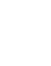
\includegraphics[width=0.17\textwidth]
		{figures/iterationSpace}\label{fig:f21}}
	%
	\hfill
	%
	\subfloat[cubic decomposition]{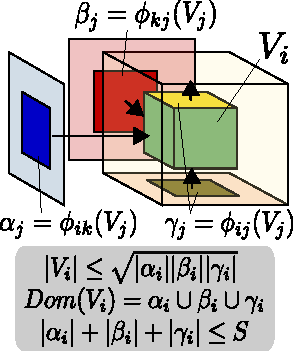
\includegraphics[width=0.14\textwidth]
		{figures/mmm_reuse_1}\label{fig:f22}}
	%
	\hfill
	%
	\subfloat["flat" decomposition]{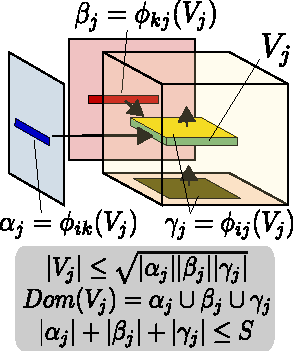
\includegraphics[width=0.14\textwidth]
		{figures/mmm_reuse_2}\label{fig:f23}}
	%
	% 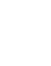
\includegraphics[width=0.26\textwidth]{figures/iterationSpace}
	\caption{\label{fig:f21} An MMM CDAG forming a 3D 
		iteration 
		space $\mathcal{V} \subset \mathbb{Z}^3$. An input matrix A (blue 
		vertices) 
		is represented as 
		its projection $\alpha = \phi_{ik}(\mathcal{V})$
		on 
		an \textbf{ik} plane - similarly, an input matrix B (red vertices) is a 
		projection $\beta = \phi_{kj}(\mathcal{V})$ on the \textbf{kj} plane 
		and an 
		output 
		matrix C (light yellow) 
		is a 
		projection $\gamma = \phi_{ij}(\mathcal{V})$ on the \textbf{ij} plane. 
		Each 
		vertex 
		in this iteration space 
		(except of the vertices in the bottom layer) has three parents - blue, 
		red, 
		and yellow and one yellow child (except of vertices in the top layer). 
		$\alpha \cup \beta \cup \gamma$ form the dominator set $Dom(V_i)$.  
		subcomputation $V_i \subset \mathcal{V}$ of an $S$-partition must 
		satisfy 
		$|Dom(V_i)| = |\alpha| + |\beta| + |\gamma| \le S$ (number of inputs 
		must 
		be 
		smaller than $S$. \ref{fig:f22} 
		optimal surface to volume subset shape. Note that in a subsequent 
		subset computation only one of the three planes (blue, red or yellow) 
		can 
		be reused. \ref{fig:f23} the optimal subset shapes when 
		data reuse is considered. Observe that even though $|V_i| > |V_j|$, but 
		$|V_i|/(|\alpha_i| + |\beta_i|) < |V_j|/(|\alpha_j| + |\beta_j|)$.}
	\label{fig:iterationSpace}
\end{figure}
% \begin{figure}
%  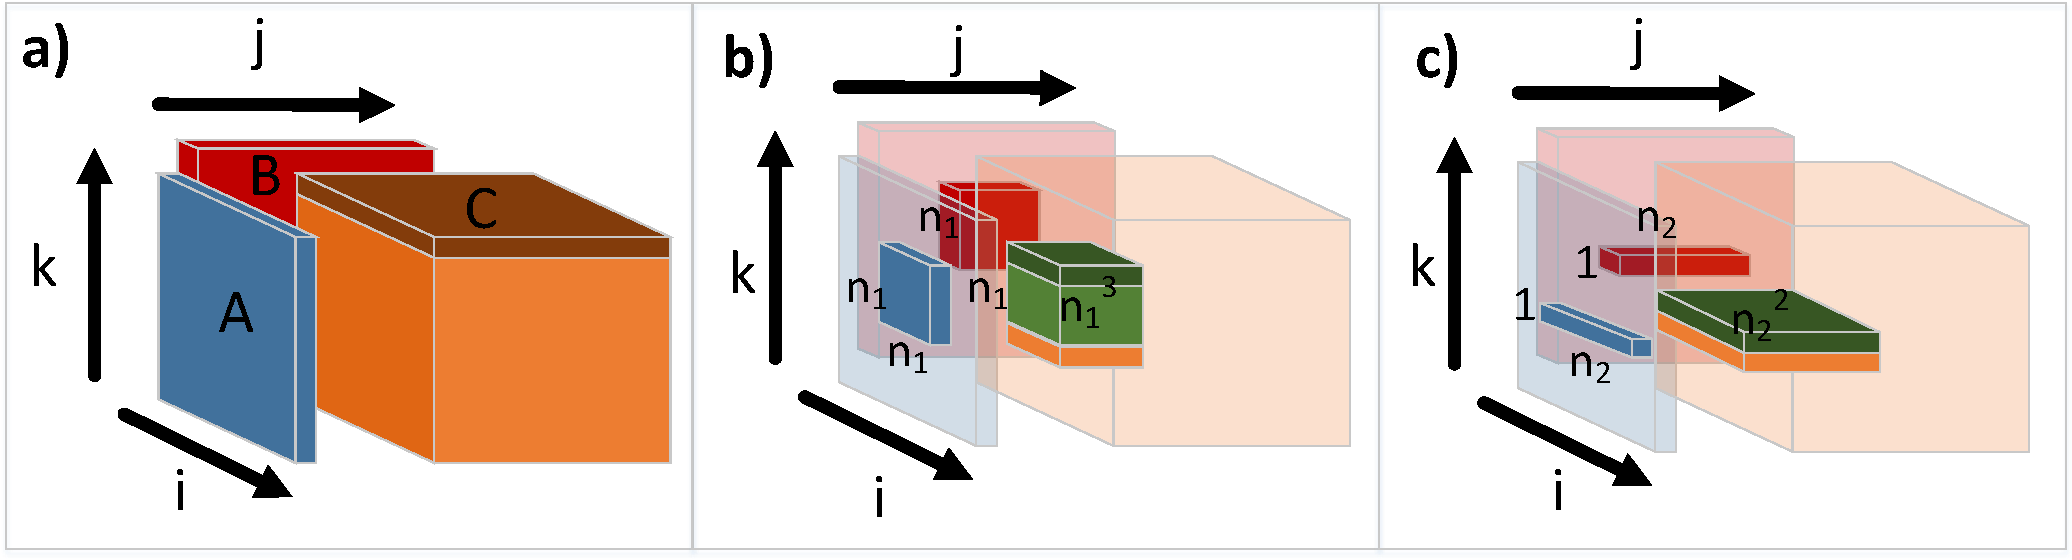
\includegraphics[width=\columnwidth]{figures/mmm_reuse}
%  \caption{MMM subset shape. a) 
%    geometric interpretation of $C = A B$ (orange cube represents 
%    3-dimensional iteration space of partial sums, matrix C is formed by 
%    reduction over dimension $k$ - represented by dark orange plane). b) 
%    optimal surface to volume subset shape. Note that in a subsequent 
%    subset computation only one of the three planes (blue, red or dark 
%    green) can be reused. c) the optimal subset shapes when 
%    data reuse is considered. In b) and c) blue, red, and orange surfaces 
%    form the dominator set, whereas dark green surface is the 
%    minimum set.}
%  \label{fig:mmmreuse}
%\end{figure}

To show why Lemma 2 gives a tighter bound than Lemma 1, consider the MMM CDAG
\mac{---> a CDAG of MMM}.  We can draw it in a 3D iteration space~\cite{tiling}
(Figure~\ref{fig:iterationSpace}), with \textbf{i},\textbf{j},\textbf{k} as
orthonormal vectors spanning it \mac{---> orthonormal spanning vectors}. Then,
an $S$-partition is a decomposition of this space into subcomputations whose
number of inputs (parents in matrices A, B and C \mac{what is a parent in a
	matrix? very confusing}) is smaller than $S$. The geometric interpretation 
	of
this input set is the union of projections of the subset onto planes
\textbf{ij}, \textbf{ik} and \textbf{kj}~\cite{loomisApplied}.

Assume that each subcomputation forms a cuboid $[a \times b \times c]$ in this
iteration space (we actually prove it in~\cref{sec:seqScheduling}) and its
faces form its input (\mac{the !!!} dominator set).  Now according to \mac{--->
	Based on} Lemma~\ref{eq:redbluebound}, we construct a $2S$-partition with a
minimal cardinality, generating subcomputations of a cubic ($a = b = c$) shape
(Figure~\ref{fig:iterationSpace} b), with a cube side $a = \sqrt{2S/3}$.  Such
schedule will perform $2a^2 \frac{n^3}{a^3} =
\sqrt{\frac{3}{2}}\frac{2N^3}{\sqrt{S}}$ I/O operations. 

Now, the question is: what is the size of a maximum reuse $R(S)$? Observe that
only one of three faces of this cuboid can be reused (used by a subsequent
subcomputation while still being in fast memory). This observation will help us
derive in (~\cref{sec:seqScheduling}) a "flat" shape (Figure 
\ref{fig:iterationSpace}
c) which performs $\frac{2N^3}{\sqrt{S}}$ I/O operations - an $\sqrt{3/2}$
improvement.



\end{document}




\end{document}
